\chapter{Literature review}

\section*{Introduction}
%? Quel est l'objectif de ce chapitre ? Comment se construit-il ?
This chapter presents and discusses previous conducted works related to the three research questions driving this dissertation.
The research questions previously identified are:

\begin{enumerate}
    \item What can decision-relevant information from social media be processed automatically?
    \item How can the actionable information available on social be automatically retrieved during crisis response?
    \item What challenges are faced by an information system dedicated to crisis management that embeds machine learning models?
\end{enumerate}

Each research question has its dedicated section.
Each section presents the evolution of the associated fields and the trends that have guided their development.
The review of this literature allows for the identification of research directions for the following chapters.
The remainder of this section presents the methodology used for the literature review and the research hypotheses.

% TODO Ajouter la collection d'articles de Leysia Palen https://docs.google.com/document/d/1sP6TsuPSCSgoHZKEM7fqZ8BXZccv3JS8TobRJXEHD7Q/edit
\subsection*{Methodology}
A mixed approach was taken to capture the evolution of work related to each research question
First, the scope of the literature review is defined through research hypotheses.
Once these hypotheses are created, the queries are made on Scopus~\footnote{https://www.scopus.com/}, a bibliographic database.

The results obtained are then be analyzed from several angles.
First, the evolution of the volume of publications returned by the query to attempt to represent the interest in the topic.
Secondly, an analysis of the keywords is made through VOSviewer~\footnote{https://www.vosviewer.com/} "a software tool for constructing and visualizing bibliometric networks."
Especially VOSviewer allows visualizing bibliographic features such as the networks of authors or keywords.
The keywords used by the different articles fetched by request provide valuable insights into the evolution of a given field, especially its interdisciplinary aspect.
Finally, the results of the most cited articles are discussed.
This methodology should make it possible to show the evolution of the scientific community's interest in the topics explored.

\subsection*{Hypotheses}
This sub-section establishes the scope of the research conducted in the rest of the chapter.
First, the only data source considered is social media.
As mentioned in the previous chapter, social media data present a set of specificities that differ from other data sources such as newspapers.
Secondly, the literature review is scoped to the crisis management context.
Finally, it is assumed that facilitating decision-making necessarily improves disaster response.
Thus, the following working hypotheses delimit the work presented.

\begin{enumerate}
    \item Social media data: social media data have a low ratio of information/noise.
    \item Crisis management: the crisis management context is particular, and this manuscript focuses on the response phase and its context.
    \item Improving the decision-making process leads to better disaster response.
\end{enumerate}

These hypotheses guide the literature review around the research questions outlined above.
Thus, the first section presents previous works on systems that automatically process social media for crisis response.
Then, the second section explores the first research question and develops on previous representations of information created.
The third and final section overlooks the different attempts to process social media data using Natural Language Processing methods.
As the third research question also refers to systems for processing social media data automatically, it shares the insights of the first section.

\section{Information systems for crisis response fed with social media data}
% * Done
The first chapter identified the opportunities offered by social media to support crisis response.
Many researchers explored these opportunities and proposed various systems and architectures to process social media data automatically.
The ultimate goal of these researches is to provide valuable insights to decision-makers.
This first part of the literature review highlights the main systems built for this purpose.
The research question this part aims to answer is: \emph{What are the existing social media processing system developed for crisis response over the years?}

The request run on the Scopus database is broken down in table~\ref{table:request-information-systems}.
It returns 96 documents published between 2011 and 2021.
The beginning of this domain of research corresponds to the democratization of social media, with the development of social media platforms happening during the 2000-2010 period (Figure~\ref{literature:crisis-informatic-hist}).
Naturally, the field has developed, driven by the need of crisis management organizations and the public interest benefit it promises.

\begin{table}[bht]
    \centering
    \caption{Overview of the bibliographic request related to information systems.}
    \tabulinesep=1.2mm
    \begin{tabu} to \textwidth {X[0.5,r]X[1,m]X[1,m]}
        Type of request & Keywords                                                                                                                                     & Explaination                                                                                                          \\ [0.5ex]
        \toprule
        SUBJAREA        & \textit{comp}                                                                                                                                & Articles in the Computer Science domain                                                                               \\
        TITLE-ABS-KEY   & \textit{crisis management} OR \textit{crisis response} OR \textit{contingency} OR \textit{disaster response} OR \textit{disaster management} & Articles related to crisis management                                                                                 \\
        TITLE-ABS-KEY   & \textit{system} AND \textit{processing}                                                                                                      & And concern systems processing information                                                                            \\
        TITLE-ABS-KEY   & \textit{social media} OR \textit{twitter}                                                                                                    & Using social media sources. Twitter is specifically indicated because of its prevalent use in the research community. \\
        EXCLUDE-DOCTYPE & \textit{re} OR \textit{cr}                                                                                                                   & Reviews and conference tracks introductions are excluded                                                              \\
        \bottomrule
    \end{tabu}
    \label{table:request-information-systems}
\end{table}


\begin{figure}[thb]
    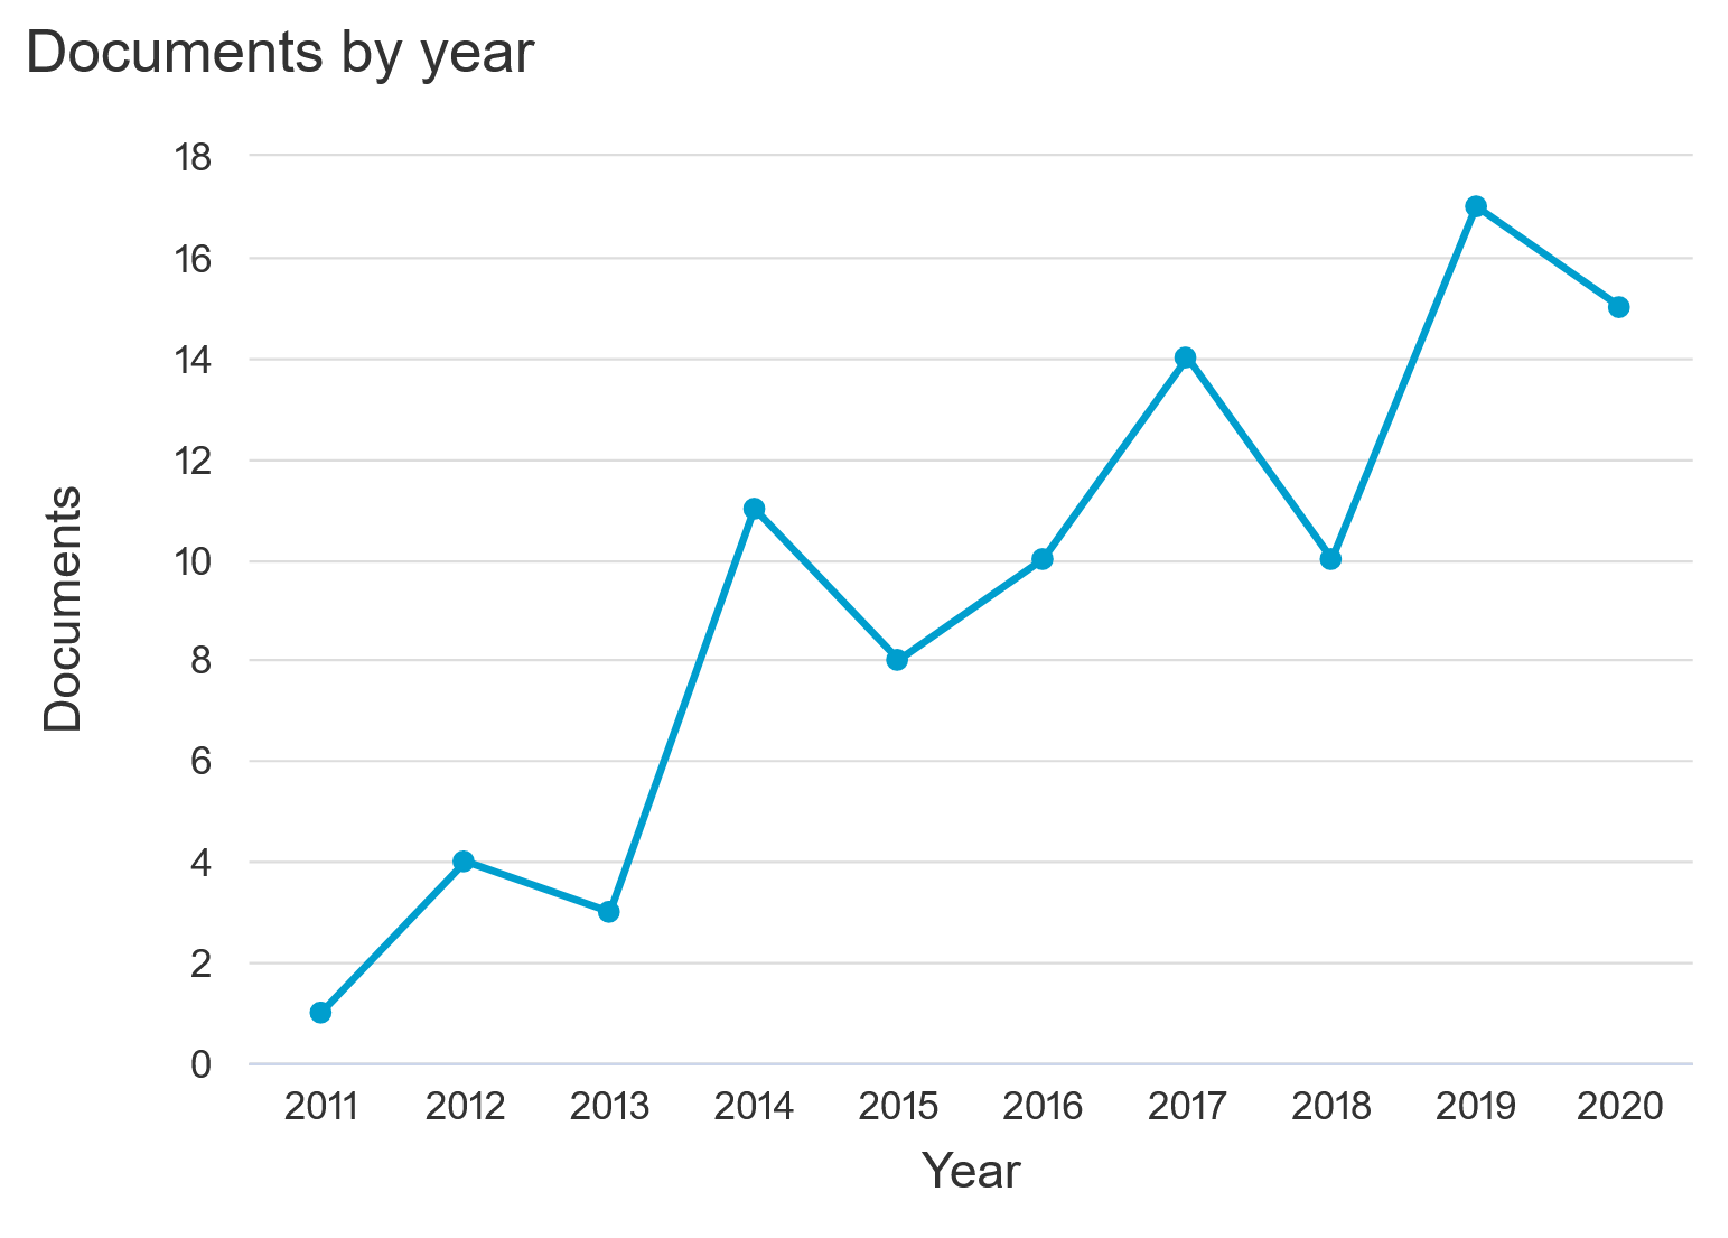
\includegraphics[width=\textwidth]{figures/chap-2/crisis-informatic-hist.pdf}
    \caption{Timeline of the volume of contributions per years for the crisis informatic domain. The year 2021 is excluded because the year is not complete at the time of writing.}
    \label{literature:crisis-informatic-hist}
\end{figure}

The network provided by VOSviewer (Figure~\ref{literature:crisis-informatic-overlay}) does not reveal any significant cluster of keywords.
The youth of the domain can explain the structure observed, as no prominent direction as been created yet.
However, the publication timeline (represented by the color variation) provides insights into the direction of the domain.
Years around 2016 mainly were focused on data analyses of the different datasets available.
Then, the following years saw the development of more and more automation.
Artificial intelligence, machine learning, and natural language processing appeared in that chronological order, coinciding with the progress made in these areas.
More recently, deep learning models to process text and images are appearing, as well as new opportunities created by the internet of things and the development of the concept of smart cities.
It is also worth noting that social and computer sciences are blended in this big picture.

\begin{landscape}
    \begin{figure}[hp]
        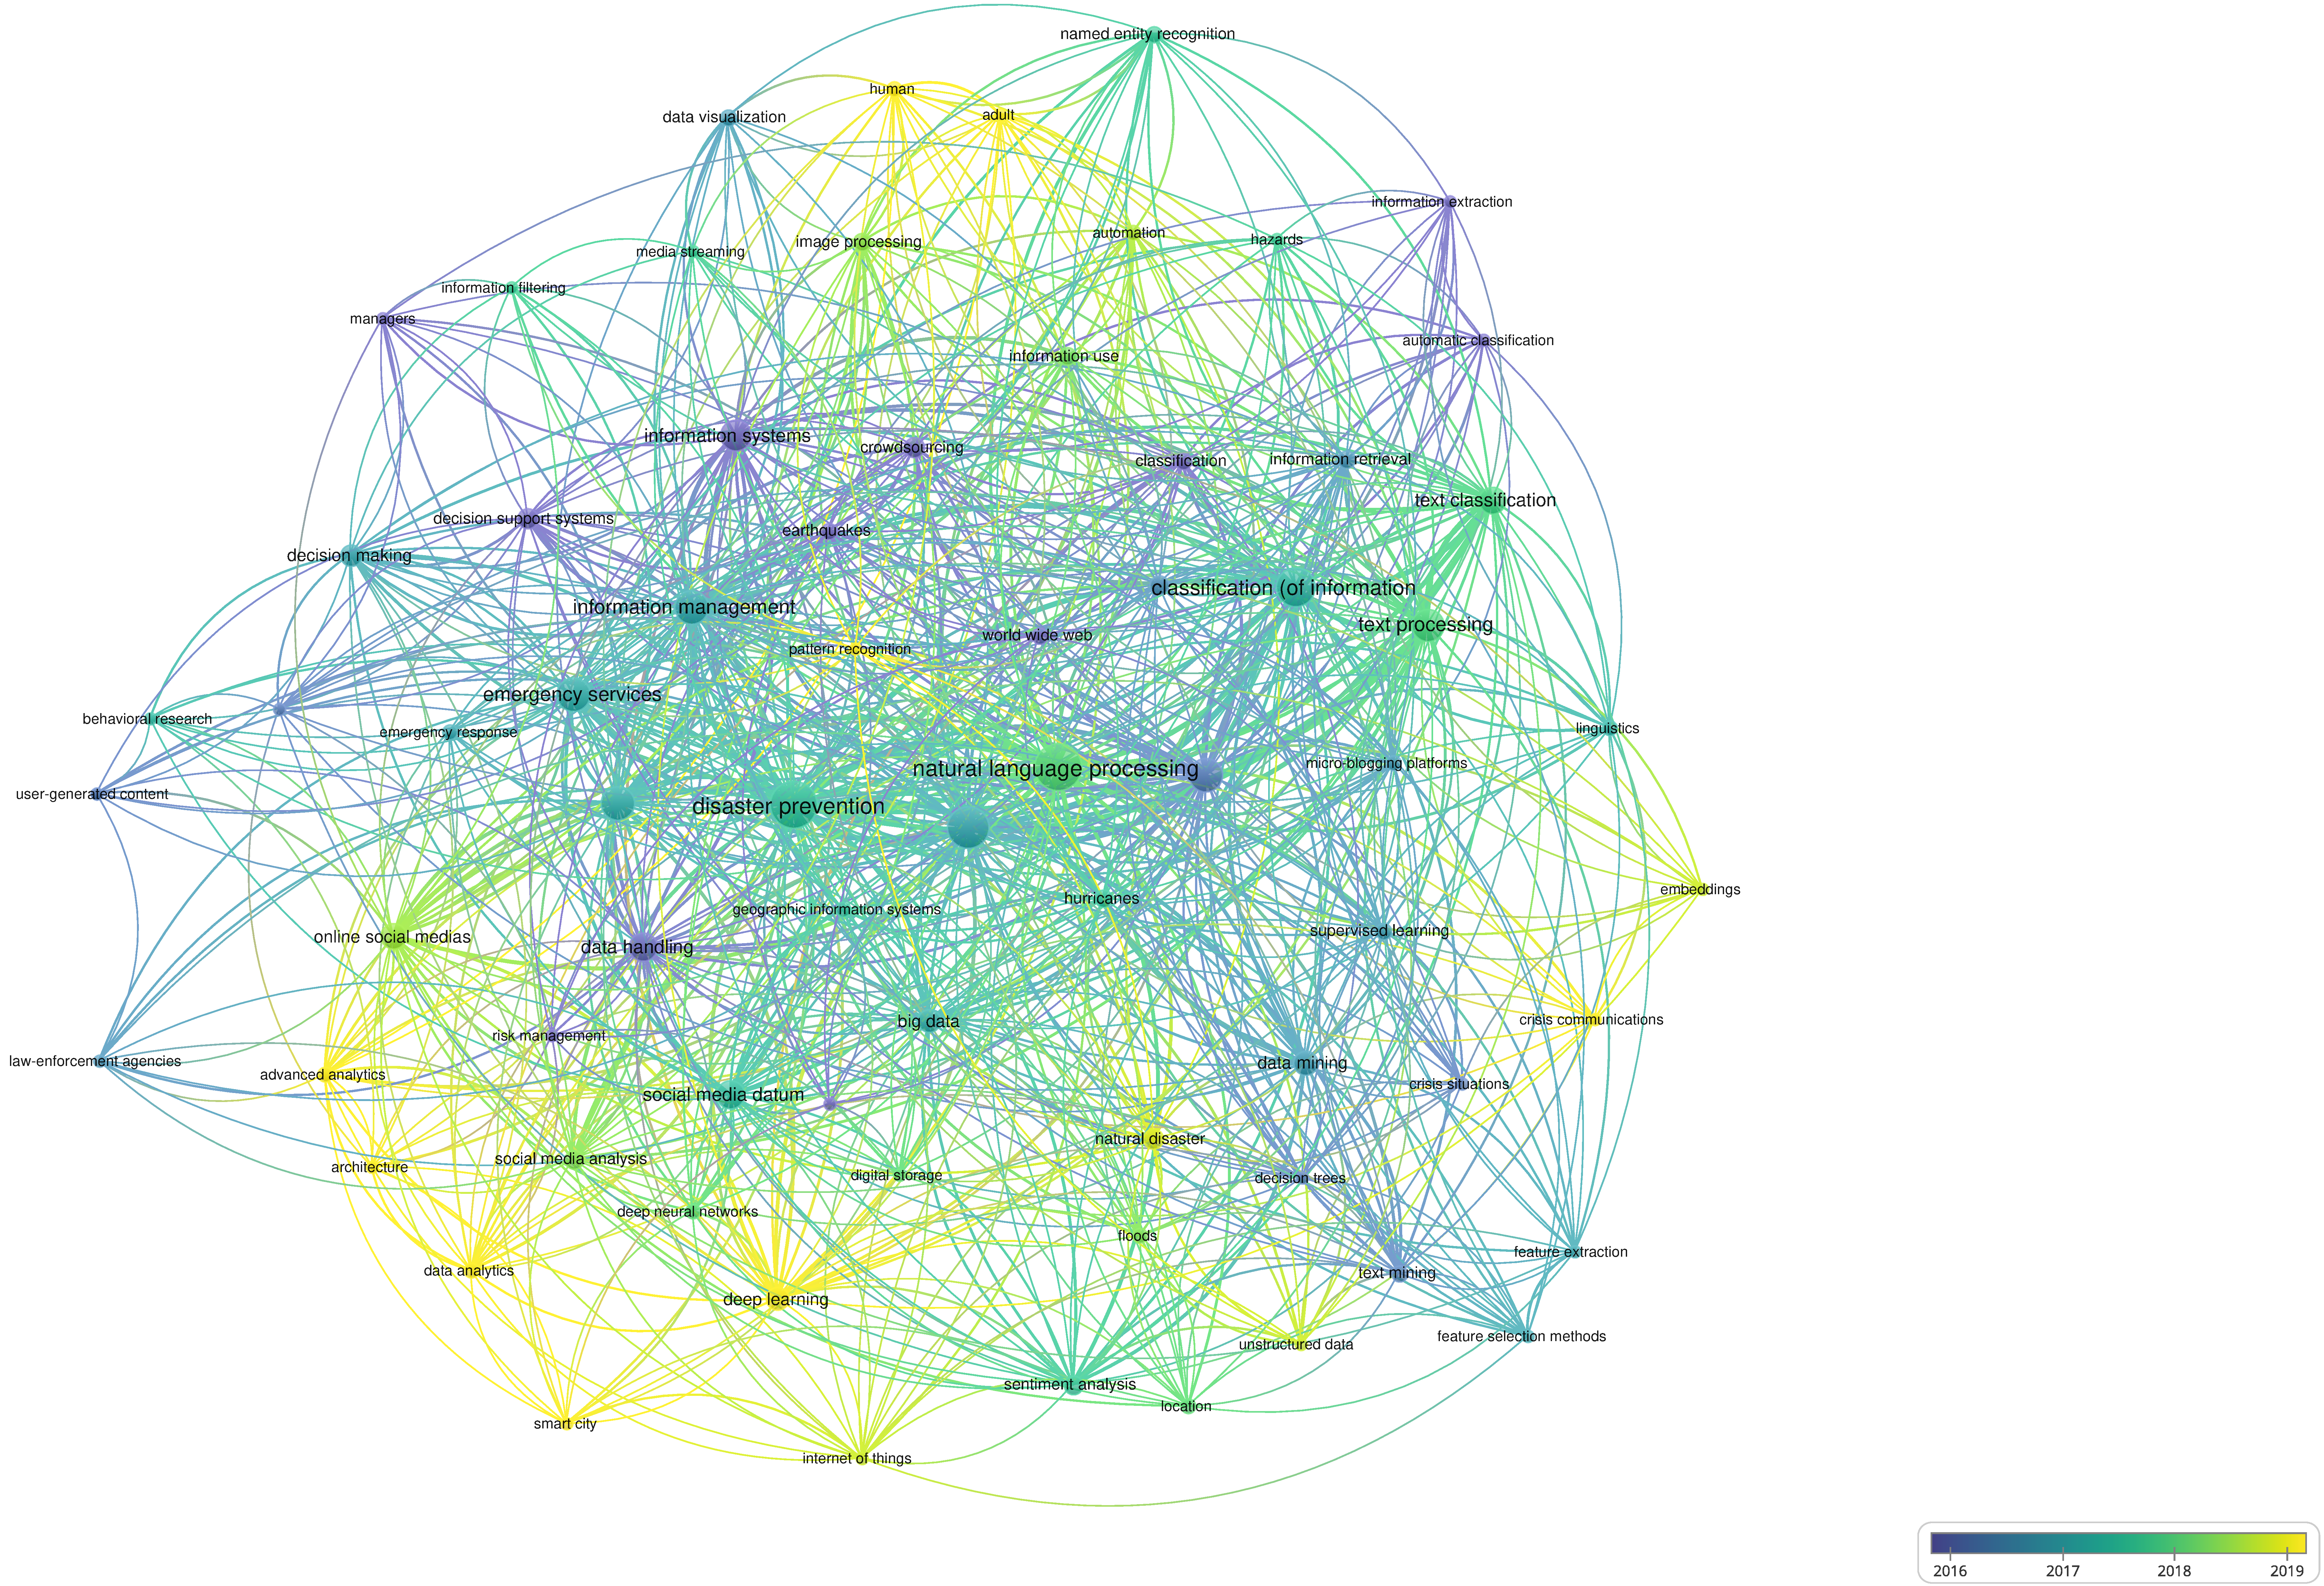
\includegraphics[width=\paperwidth,height=\paperheight,keepaspectratio]{figures/chap-2/crisis-informatic-overlay.pdf}
        \caption{Distribution of keywords with more than 3 occurrences among the articles from the query on crisis informatics. }
        \label{literature:crisis-informatic-overlay}
    \end{figure}
\end{landscape}

The bar diagram (Figure~\ref{literature:crisis-informatic-bar}) provides a representation of the distribution of the occurrences of the different keywords.
From the most used keywords, two areas of interest seem to emerge.
The first one is the automatic processing of social media data.
The type of data appears to be primarily textual, according to the prevalent use of \emph{natural language processing} and \emph{text processing} is no more important than the use of this automation.
\emph{Disaster prevention}, \emph{situation awareness}, \emph{information management} and \emph{emergency services} highlight the importance of the applications of the results.

\begin{figure}[thb]
    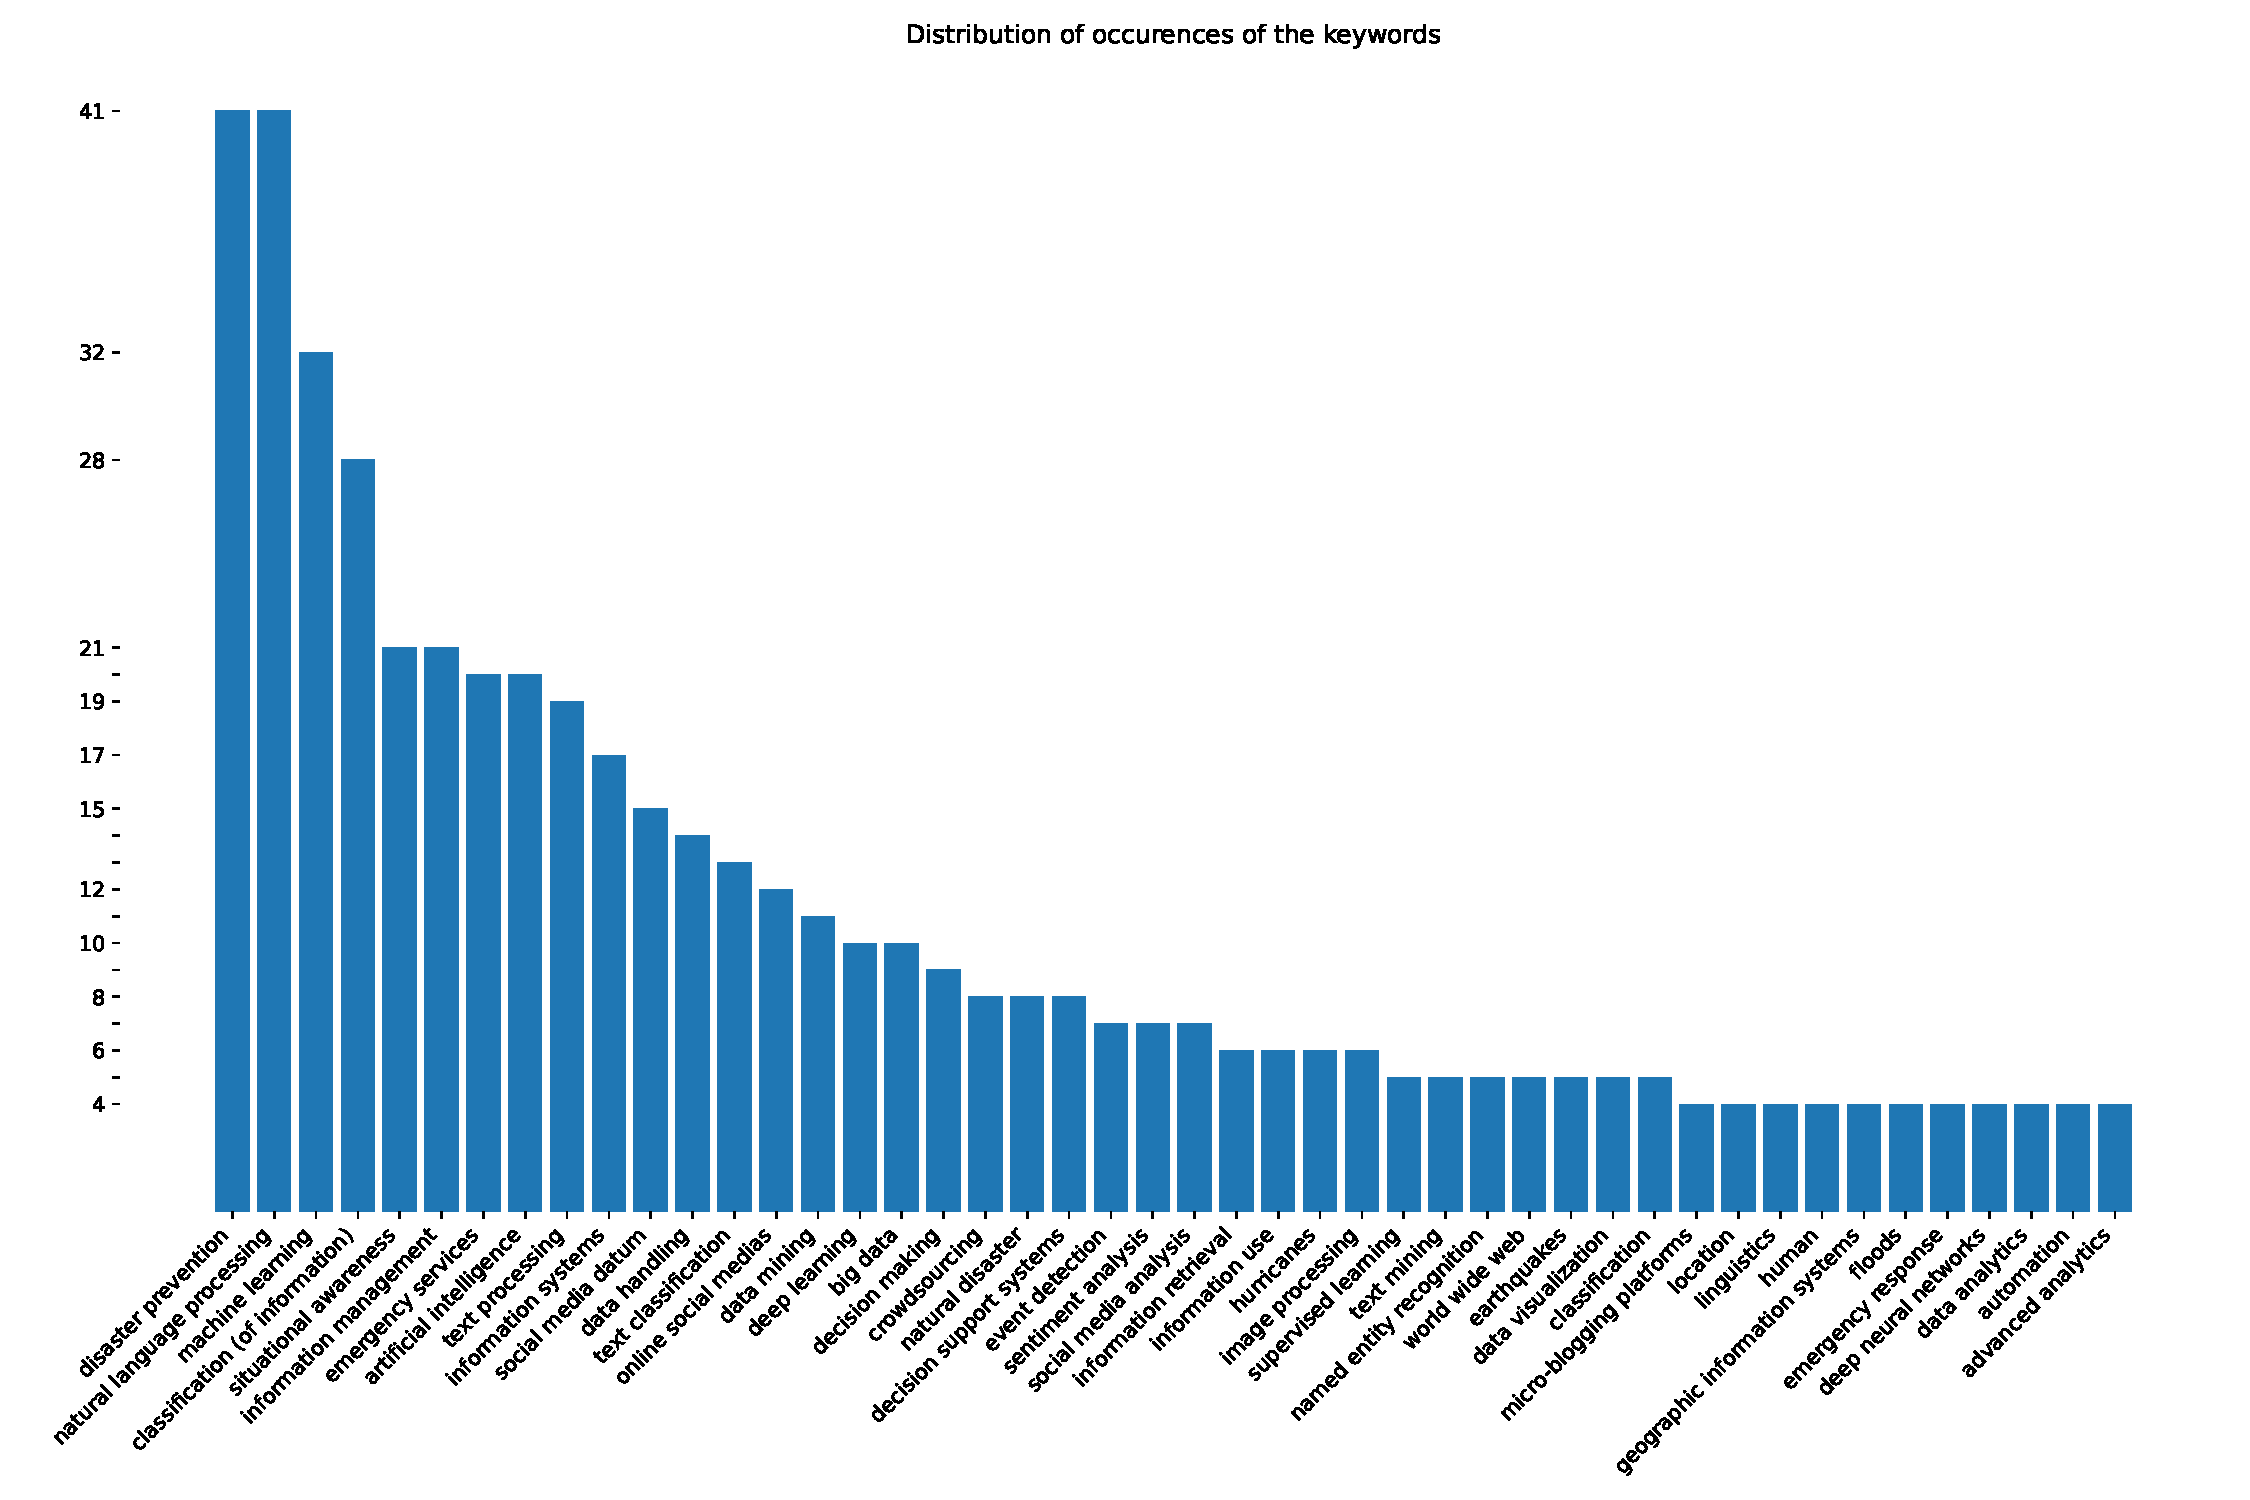
\includegraphics[width=\textwidth]{figures/chap-2/crisis-informatic-bar.pdf}
    \caption{Distribution of keywords with more than 3 occurrences among the articles from the query on crisis informatics. }
    \label{literature:crisis-informatic-bar}
\end{figure}

As mentioned in the first chapter, automatically processing the content of social media to extract information is a new and promising scientific venue.
Thus, many attempted to create systems to achieve this goal, proposing features to improve usability.
Table~\ref{table:crisis-informatic-main-articles} presents the results of the previous query that mention a processing system that uses social media as a data source and that has been cited at least ten times are shown.
The right column of the table summarizes the main features proposed by the authors.

Among the features identified, the trend towards automation observed earlier is clear.
The first iterated systems were mainly relying on crowdsourcing to identify relevant information from messages posted on social media
\parencite{schulzCrisisInformationManagement2012, backfriedOpenSourceIntelligence2012,imranAIDRArtificialIntelligence2014}.
The following works were interested in automating the previous tasks to reduce the dependence on human resources and improve massive data processing.
Problems related to the detection of occurence of events and their related information on social media, have been explored using different approaches \parencite{imranAIDRArtificialIntelligence2014,middletonRealtimeCrisisMapping2014,avvenutiEARSEarthquakeAlert2014, gibsonCombiningBigSocial2014}.
In parallel, experiments were conducted to identify the best ways to organize and disseminate the information obtained \parencite{middletonRealtimeCrisisMapping2014,huangDisasterMapperCyberGISFramework2015,avvenutiPullingInformationSocial2016,grunder-fahrerTopicsTopicalPhases2018}.
Building on its successes, the field has continued to develop by relying on other available data formats and in particular images \parencite{alamImage4ActOnlineSocial2017,nguyenAutomaticImageFiltering2017,agarwalCrisisDIASMultimodalDamage2020}.
Beyond the data, new questions have emerged, following feedback from the emergency departments involved in the experiments.
The detection of sub-events and the different concerns of the impacted population is added to the results of previous works \parencite{wuStreamExplorerMultiStageSystem2018,raginiBigDataAnalytics2018,grunder-fahrerTopicsTopicalPhases2018}.
More recently, teams with a broader vision are interested in the integration of such systems within smart cities \parencite{shahDisasterResilientSmart2019}.
The multiplication of sources and formats naturally leads to the need for unified processing methods for data and fusion of information obtained by the different channels \parencite{alamDescriptiveVisualSummaries2020}.

This introductory section presented previous works around crisis informatics.
More particularly, it highlighted the development of the field over time.
This development is directly reflected in the different systems developed and their features.
An interesting trend to note is the move towards more and more automation in systems.
First, using crowdsourcing for initial data labeling, the following systems used machine learning to classify the data into different categories.
Currently, automation was further extended to other valuable data types and ways to merge the information acquired.

\begin{table}[bh]
    \centering
    \tabulinesep=1.2mm
    \caption{Articles retrieved from the previous request which propose social media processing systems or methods with at least 10 citations.}
    \begin{tabu} to \textwidth {X[3,m]X[1.5,m]X[5,m]}
        Reference                                       & Type of event studied & Features                                                 \\ [0.5ex]
        \toprule
        \cite{schulzCrisisInformationManagement2012}    & None                  & Crowdsourcing                                            \\
        \cite{backfriedOpenSourceIntelligence2012}      & None                  & Crowdsourcing, Automatic processing                      \\
        \cite{imranAIDRArtificialIntelligence2014}      & None                  & Crowdsourcing, Information categories, Message filtering \\
        \cite{middletonRealtimeCrisisMapping2014}       & None                  & Common Operational Picture, Location inference           \\
        \cite{avvenutiEARSEarthquakeAlert2014}          & Earthquake            & Event detection                                          \\
        \cite{gibsonCombiningBigSocial2014}             & None                  & Formal concept analysis, Rule-based method               \\
        \cite{glasgowOurGriefUnspeakable2014}           & None                  & Death-related content detection                          \\
        \cite{huangDisasterMapperCyberGISFramework2015} & None                  & Big Data, Common Operational Picture                     \\
        \cite{avvenutiPullingInformationSocial2016}     & Earthquake, Flooding  & Event detection, Message filtering, Disaster management  \\
        \cite{alamImage4ActOnlineSocial2017}            & None                  & Image processing, Infrastructure damage                  \\
        \cite{fersiniEarthquakeManagementDecision2017}  & Earthquake            & Message filtering, Information management                \\
        \cite{nguyenAutomaticImageFiltering2017}        & None                  & Image processing, De-duplication, Image filtering        \\
        \cite{raginiBigDataAnalytics2018}               & Flooding              & Sentiment analysis                                       \\
        \cite{shahDisasterResilientSmart2019}           & Earthquake, Tsunami   & Smart Cities, IoT integration                            \\
        \cite{grunder-fahrerTopicsTopicalPhases2018}    & None                  & Topic modeling, Disaster management                      \\
        \cite{wuStreamExplorerMultiStageSystem2018}     & None                  & Subevent detection, Clustering                           \\
        \cite{agarwalCrisisDIASMultimodalDamage2020}    & None                  & Damage identification, Severity detection                \\
        \cite{alamDescriptiveVisualSummaries2020}       & Hurricane             & Information fusion                                       \\
        \bottomrule
    \end{tabu}
    \label{table:crisis-informatic-main-articles}
\end{table}

\section{Decision-making in crisis situation}
This part of the literature review explores the bibliographic context around the first research question: \emph{What can decision-relevant information from social media be processed automatically?}
Decision-making is at the heart of the response during a disaster.
Ideally, the right decisions need to be made at the right time.
This expectation is theoretical.
This section is split into three parts.
The first part presents the previous attempts to represent the context of crisis management.
The second part highlights the challenges faced by decision-makers when responding to disasters.
The third and final part refines the previous findings on those which consider social media.

\subsection{Organization of information during crises: crisis models}
\label{sec:lit-information-models}
With the advent of computers to delegate tasks, many have thought of charging some parts of crisis management to machines.
However, in order to delegate these tasks to computers, they must first be provided with a representation of these tasks.
In the context of crisis management, these are representations of the environment of this management.
These representations will be called crisis models in this dissertation.
Two paths to represent crisis' concepts have been taken: ontologies and metamodels.
Ontologies and metamodels have very close definitions.
Both methods aim at creating a controlled vocabulary to define the entities and their relations in a given domain.
These two methods differ in what they seek to produce \parencite{assmannOntologiesMetamodelsModeldriven2006}.
On the one hand, ontologies \emph{define} concepts, providing a vocabulary and a grammar for manipulating the concepts studied.
On the other hand, metamodels \emph{represent} computationally the studied concepts, preferably using a standard modeling language.
More precisely, they seek to represent the information associated with the concept.
Therefore, metamodels and information models will both be used interchangeably in the following.
Standard modeling languages such as the Unified Modeling Language (UML) are preferred as they ease the distribution and development of these representations.
As the backbone of model-driven engineering, Metamodels tend to be developed with interoperability between different systems in mind.
Ontologies and metamodels have been both applied to crisis management.
Due to the tremendous variety induced by crises themselves, many ontologies and metamodels have been proposed to represent different aspects of crisis management.
Consequently, ontologies and information models emerged to represent the informational concepts manipulated during an emergency.
This sub-section aims at retrieving from the literature the different key informational concepts useful for decision-makers during crisis response.
The query used to explore this domain is summarized in Table~\ref{table:crisis-models}.

\begin{table}[bht]
    \centering
    \tabulinesep=1.2mm
    \caption{Overview of the bibliographic request related to crisis models.}
    \begin{tabu} to \textwidth {X[0.5,r]X[1,m]X[1,m]}
        Type of request & Keywords                                                                                                                                     & Explaination                                             \\ [0.5ex]
        \toprule
        SUBJAREA        & \textit{comp}                                                                                                                                & Articles in the Computer Science domain                  \\
        TITLE-ABS-KEY   & \textit{crisis management} OR \textit{crisis response} OR \textit{disaster management} OR \textit{contingency} OR \textit{disaster response} & Articles related to crisis management                    \\
        TITLE-ABS-KEY   & \textit{ontology} OR \textit{metamodel}                                                                                                      & And methods to represent and model information           \\
        EXCLUDE-DOCTYPE & \textit{re} OR \textit{cr}                                                                                                                   & Reviews and conference tracks introductions are excluded \\
        \bottomrule
    \end{tabu}
    \label{table:crisis-models}
\end{table}

The request returns 205 documents published between 1998 and 2021.
Figure~\ref{literature:situation-models-hist} shows the evolution of the volume of publication during this period.
According to the Scopus database, the field has emerged around 2000 and progressed over ten years to reach a plateau of fifteen articles on average per year.
The objective of this research was to identify and organize the information and knowledge used in crisis management.
As mentioned before, the final goal is to delegate part of the management of this information to computers.
For this, it is necessary to structure the required information and knowledge.

\begin{figure}[thb]
    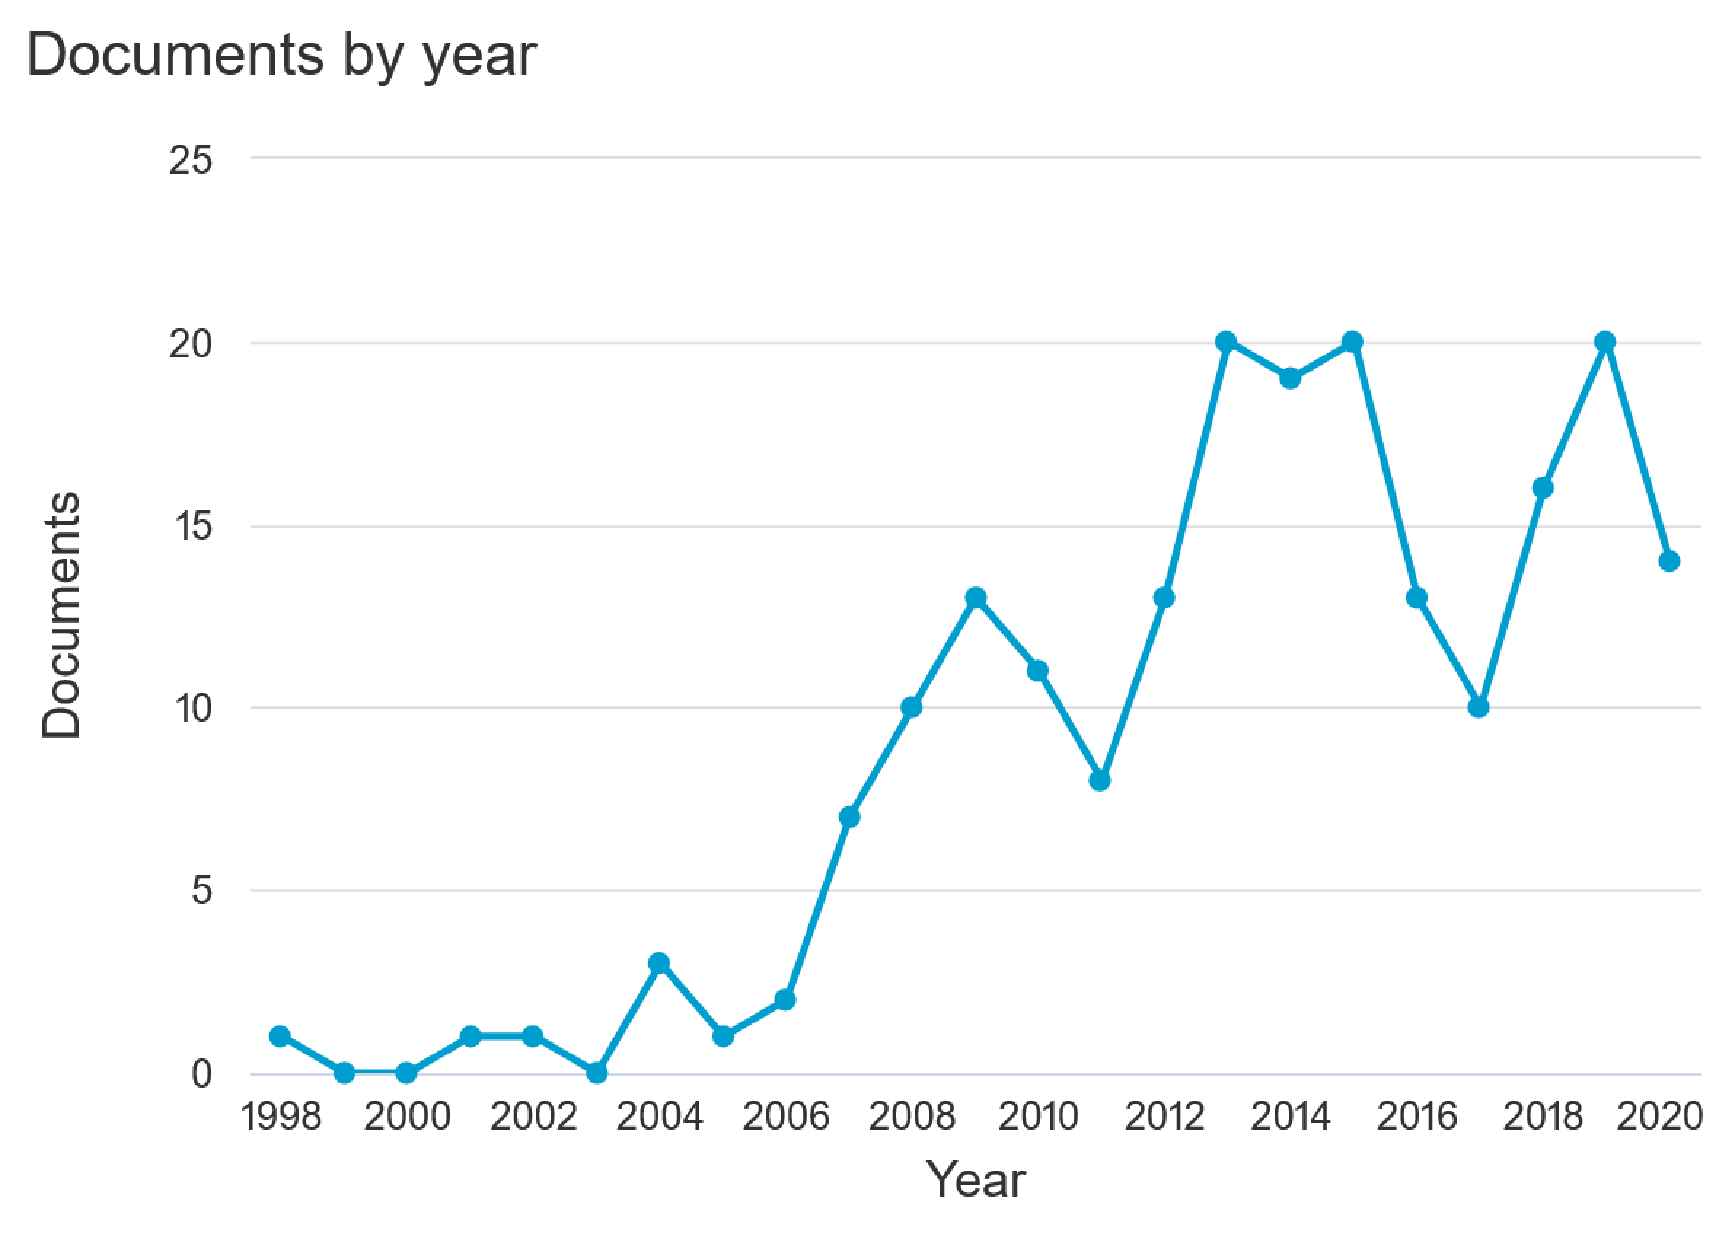
\includegraphics[width=\textwidth]{figures/chap-2/situation-models-hist.pdf}
    \caption{Timeline of the volume of contributions per years for the crisis-situation models domain. The year 2021 is excluded because the year is not complete at the time of writing.}
    \label{literature:situation-models-hist}
\end{figure}

Following the same methodology as in the previous section, Figure~\ref{literature:situation-models-overlay} provides a visual of the evolution over time of the different keywords used in the fetched articles.
The overlay indicates three clusters: a major one and two smaller ones.
The primary cluster focuses on the literature review topic, while the two smaller ones mainly refer to outlier topics (the petroleum and medical sectors).
As in the previous section, the evolution (represented by the color variation) of the keywords hints at the direction of the domain over time.

\begin{landscape}
    \begin{figure}[hp]
        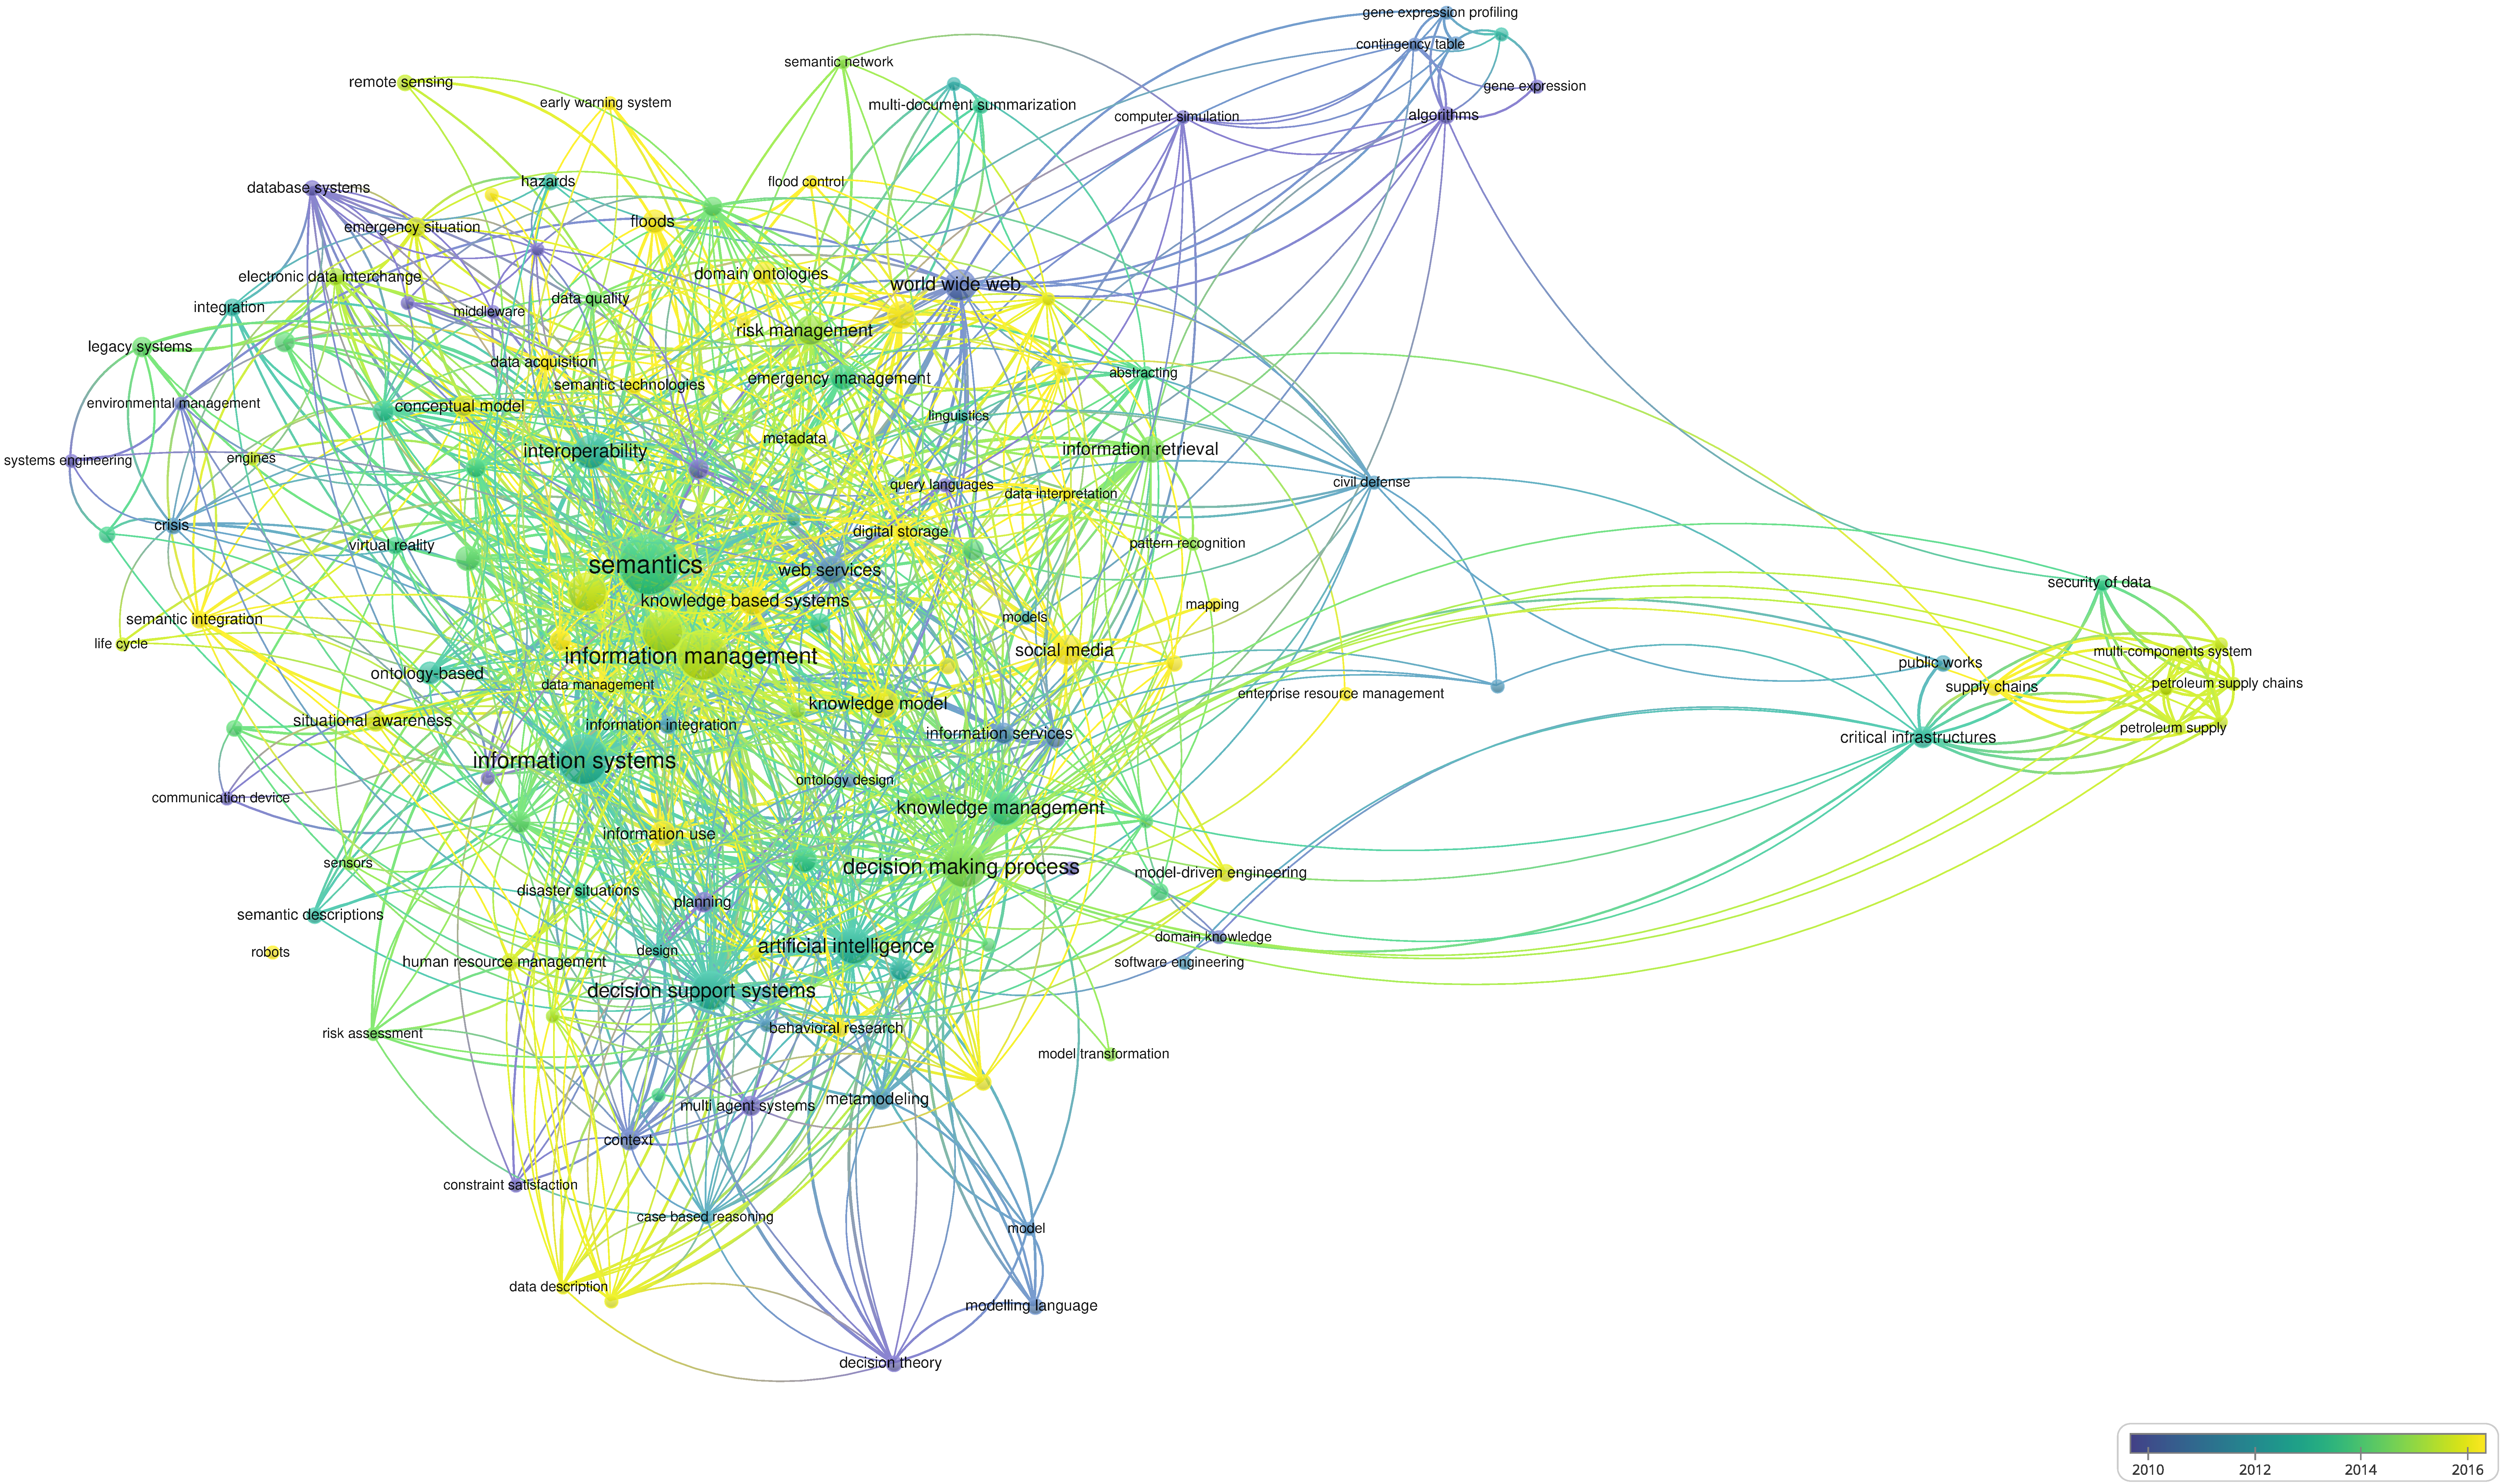
\includegraphics[width=\paperwidth,height=\paperheight,keepaspectratio]{figures/chap-2/situation-models-overlay.pdf}
        \caption{Distribution of keywords with more than 3 occurrences among the articles from the query on crisis-situation models.}
        \label{literature:situation-models-overlay}
    \end{figure}
\end{landscape}

The overlay spans from 2010 to 2016, as it filters keywords with less than three occurrences.
By cross-checking this information with the previous histogram, one understands the reason for this short period.
The histogram shows a low number of publications between 1998 and 2006, while the overlay shows an important variety of keywords used.
This pattern reflects the novelty of the domain.
The stop of the overlay in 2016 can be explained by the loss of interest in this topic from 2015.
Also, according to the histogram, the field regained interest in 2017, indicating that it is on a plateau overall.

Despite this short covered span, it is possible to identify keywords use trends similar to those in crisis informatics.
The older keywords used, such as \emph{SOA}, \emph{simulation}, \emph{multi-agent systems}, and \emph{systems engineering}, show an interest centered around the core of what we're used ontologies and metamodels for—model-driven engineering and information management.
Then, the field knew a pic of interest, as the previous histogram showed.
This period reflects on Figure~\ref{literature:situation-models-bar}, where one can observe that most of the most important keywords are located between 2012 and 2014.
As explained previously, the years between 2012 and 2014 were the most prolific.
These years were primarily focused on the idea of crisis management systems powered by artificial intelligence for decision support.
Artificial intelligence would automatically create the information representations needed by systems.
As these representations would have been written in a standard way, these systems would have adapted to new models, providing greater interoperability quickly.
After this period, the interest in the field decreases a few before coming back with new approaches.
Knowledge-based systems and knowledge management started to appear and a reborn of metamodel and ontologies creation, powered by improvements in machine learning.

\begin{figure}[thb]
    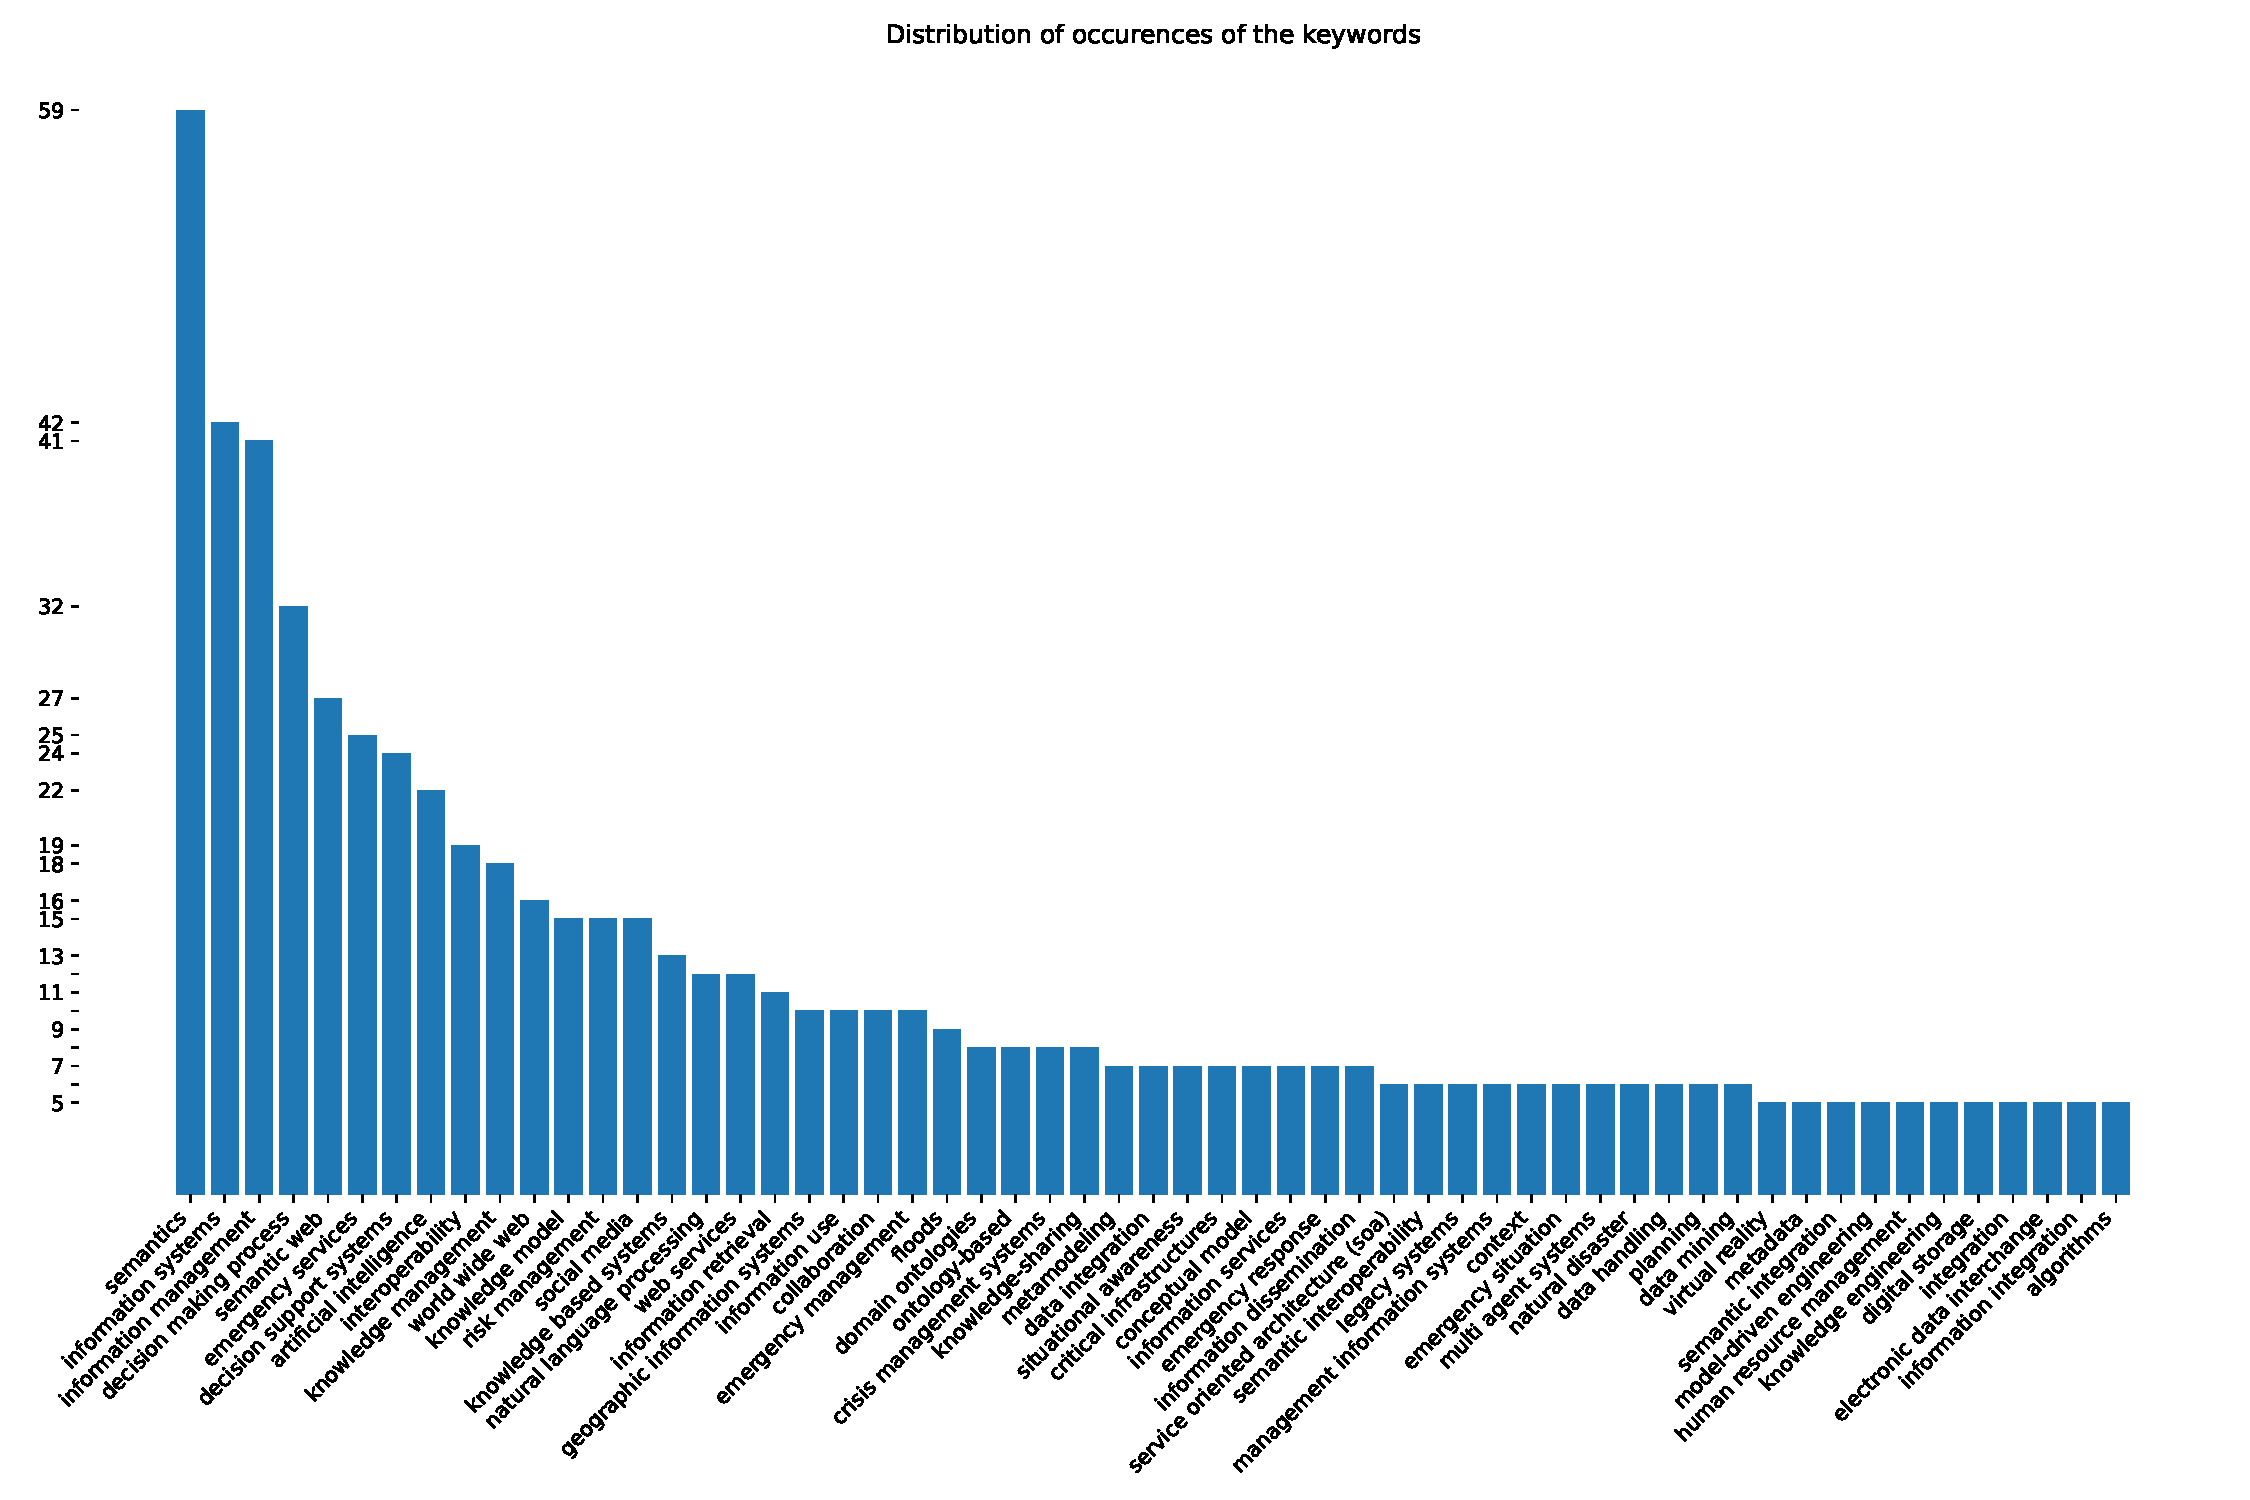
\includegraphics[width=\textwidth]{figures/chap-2/situation-models-bar.pdf}
    \caption{Distribution of keywords with more than 4 occurrences among the articles from the query on crisis-situation models.}
    \label{literature:situation-models-bar}
\end{figure}

In association with the previous qualitative review of the field, Table~\ref{table:situation-models-main-articles} presents the needs of the decision-maker identified in the articles from the previous request with at least 25 citations.
Duplicates and unrelated articles (e.g., gene ontologies) are also excluded.
This review of the main articles highlights the diversity of approaches covered by ontologies and metamodels.
Some of these ontologies are specific to certain events \parencite{xuModelingRepresentationEarthquake2014,qiuIntegratedFloodManagement2017,jungOntologydrivenSlopeModeling2015}.
While these models effectively deal with the type of disaster they are designed for, most of their concept representations do not fit with other types of events.

As mentioned in the first chapter, a proper collaboration between crisis management actors is crucial for disaster response.
Thus \textcite{benabenMetamodelItsOntology2008} and \textcite{othmanDevelopmentValidationDisaster2014} propose metamodels to represent the collaboration between several actors, independantly of the type of crisis.
The metamodel proposed by \citeauthor{benabenMetamodelItsOntology2008} is further developed in section~\hyperref[sec:crisismetamodel]{3.2.1.}

Others have also focused on emergency organizations and proposed improving their functioning.
\textcite{chouOntologyDevelopingWeb2011} proposed a way to automatically create websites to disseminate information related to an ongoing event.
As reports are an essential concern and participate in information overload, \textcite{liOntologyenrichedMultiDocumentSummarization2010} created an ontology to assist in report summarization.
Disaster management software is inherently complex.
Thus, \textcite{babitskiSoKNOSUsingSemantic2011} proposed an ontology to assist and guide the development of the software.
As disaster management systems grow, they become intricated and complex. \textcite{madniSystemsIntegrationKey2014} proposed an ontology to facilitate their integration into a functioning system of systems.

All the systems mentioned above require data.
Fortunately, sensors are excellent ways to keep emergency responders informed of specific characteristics of their environment.
\textcite{posladSemanticIoTEarly2015} and \textcite{babitskiOntologybasedIntegrationSensor2009} proposed ontologies to better integrate sensors data into crisis cells.
Finally, another type of sensor considered is humans, acting as social sensors whose data can be automatically gathered from social media platforms.
\textcite{purohitIdentifyingSeekersSuppliers2014} proposed an ontology to identify victims' requests and volunteers' capabilities from tweets.
Being able to geolocate individuals behind social media posts is critical for emergency services.
Therefore, \textcite{ghahremanlouGeotaggingTwitterMessages2014} built an ontology to help resolve this issue.

\begin{table}[bht]
    \centering
    \tabulinesep=1.2mm
    \caption{Articles retrieved from the previous request which propose social media processing systems or methods with at least 25 citations.}
    \begin{tabu} to \textwidth {X[1,m]X[3,m]}
        Reference                                               & Decision-makers needs addressed        \\ [0.5ex]
        \toprule
        \cite{benabenMetamodelItsOntology2008}                  & Collaboration                          \\
        \cite{babitskiOntologybasedIntegrationSensor2009}       & Sensor integration                     \\
        \cite{liOntologyenrichedMultiDocumentSummarization2010} & Reports summarization                  \\
        \cite{babitskiSoKNOSUsingSemantic2011}                  & Disaster management software usability \\
        \cite{chouOntologyDevelopingWeb2011}                    & Automatic web sites creation           \\
        \cite{ghahremanlouGeotaggingTwitterMessages2014}        & Location retrieval                     \\
        \cite{madniSystemsIntegrationKey2014}                   & System integration                     \\
        \cite{othmanDevelopmentValidationDisaster2014}          & Collaboration                          \\
        \cite{purohitIdentifyingSeekersSuppliers2014}           & Identify victims and volunteers        \\
        \cite{xuModelingRepresentationEarthquake2014}           & Earthquake management                  \\
        \cite{jungOntologydrivenSlopeModeling2015}              & Landslide prevention                   \\
        \cite{posladSemanticIoTEarly2015}                       & Sensor integration                     \\
        \cite{qiuIntegratedFloodManagement2017}                 & Flood management                       \\
        \bottomrule
    \end{tabu}
    \label{table:situation-models-main-articles}
\end{table}

This part identified the different approaches to model information in crisis response from a decision-maker point of view.
Yet, most of these approaches are top-down, and few conducted interviews to identify decision-makers' needs directly.
The following section focuses on articles in the literature that used a bottom-up approach to identify the needs mentioned above.

\subsection{Business needs of emergency services}
Emergency management teams are tasked with novel and complex decisions.
Information collection is one of the levers that ease decision-making and facilitate crisis management.
Knowing the different elements that hinder emergency management teams from achieving their goals and what could ease information gathering is of the utmost importance to improve crisis management.
Researchers in social sciences have been interested in studying the challenges faced.
This section aims to highlight the main issues identified in the literature.

The request summarized in Table~\ref{table:emergency-services-challenges} returns 219 documents published between 1995 and 2021.
The domain follows an increasing trend similar to the previous ones studied.
Interest in the study of emergency services has been multiplying since the 2000s.
This interest grew relatively steadily until today, where about 20 articles are published per year on the subject (Figure~\ref{literature:business-needs-hist}).

\begin{table}[bht]
    \centering
    \tabulinesep=1.2mm
    \caption{Overview of the bibliographic request related to challenges in crisis management.}
    \begin{tabu} to \textwidth {X[0.5,r]X[1,m]X[1,m]}
        Type of request & Keywords                                                                             & Explaination                                                                               \\ [0.5ex]
        \toprule
        SUBJAREA        & \textit{comp} OR \emph{soci} OR \emph{deci}                                          & Articles in either Computer Science, Social Sciences of Decision Sciences domains          \\
        TITLE-ABS-KEY   & \textit{information gathering} OR \textit{interview?}                                & Articles that conducted interviews or identified the information collected by the services \\
        TITLE-ABS-KEY   & \textit{emergency responders} OR \textit{emergency services} OR \textit{dispatchers} & Interviews were conducted by emergency services                                            \\
        EXCLUDE-DOCTYPE & \textit{re} OR \textit{cr}                                                           & Reviews and conference tracks introductions are excluded                                   \\
        \bottomrule
    \end{tabu}
    \label{table:emergency-services-challenges}
\end{table}

\begin{figure}[thb]
    \centering
    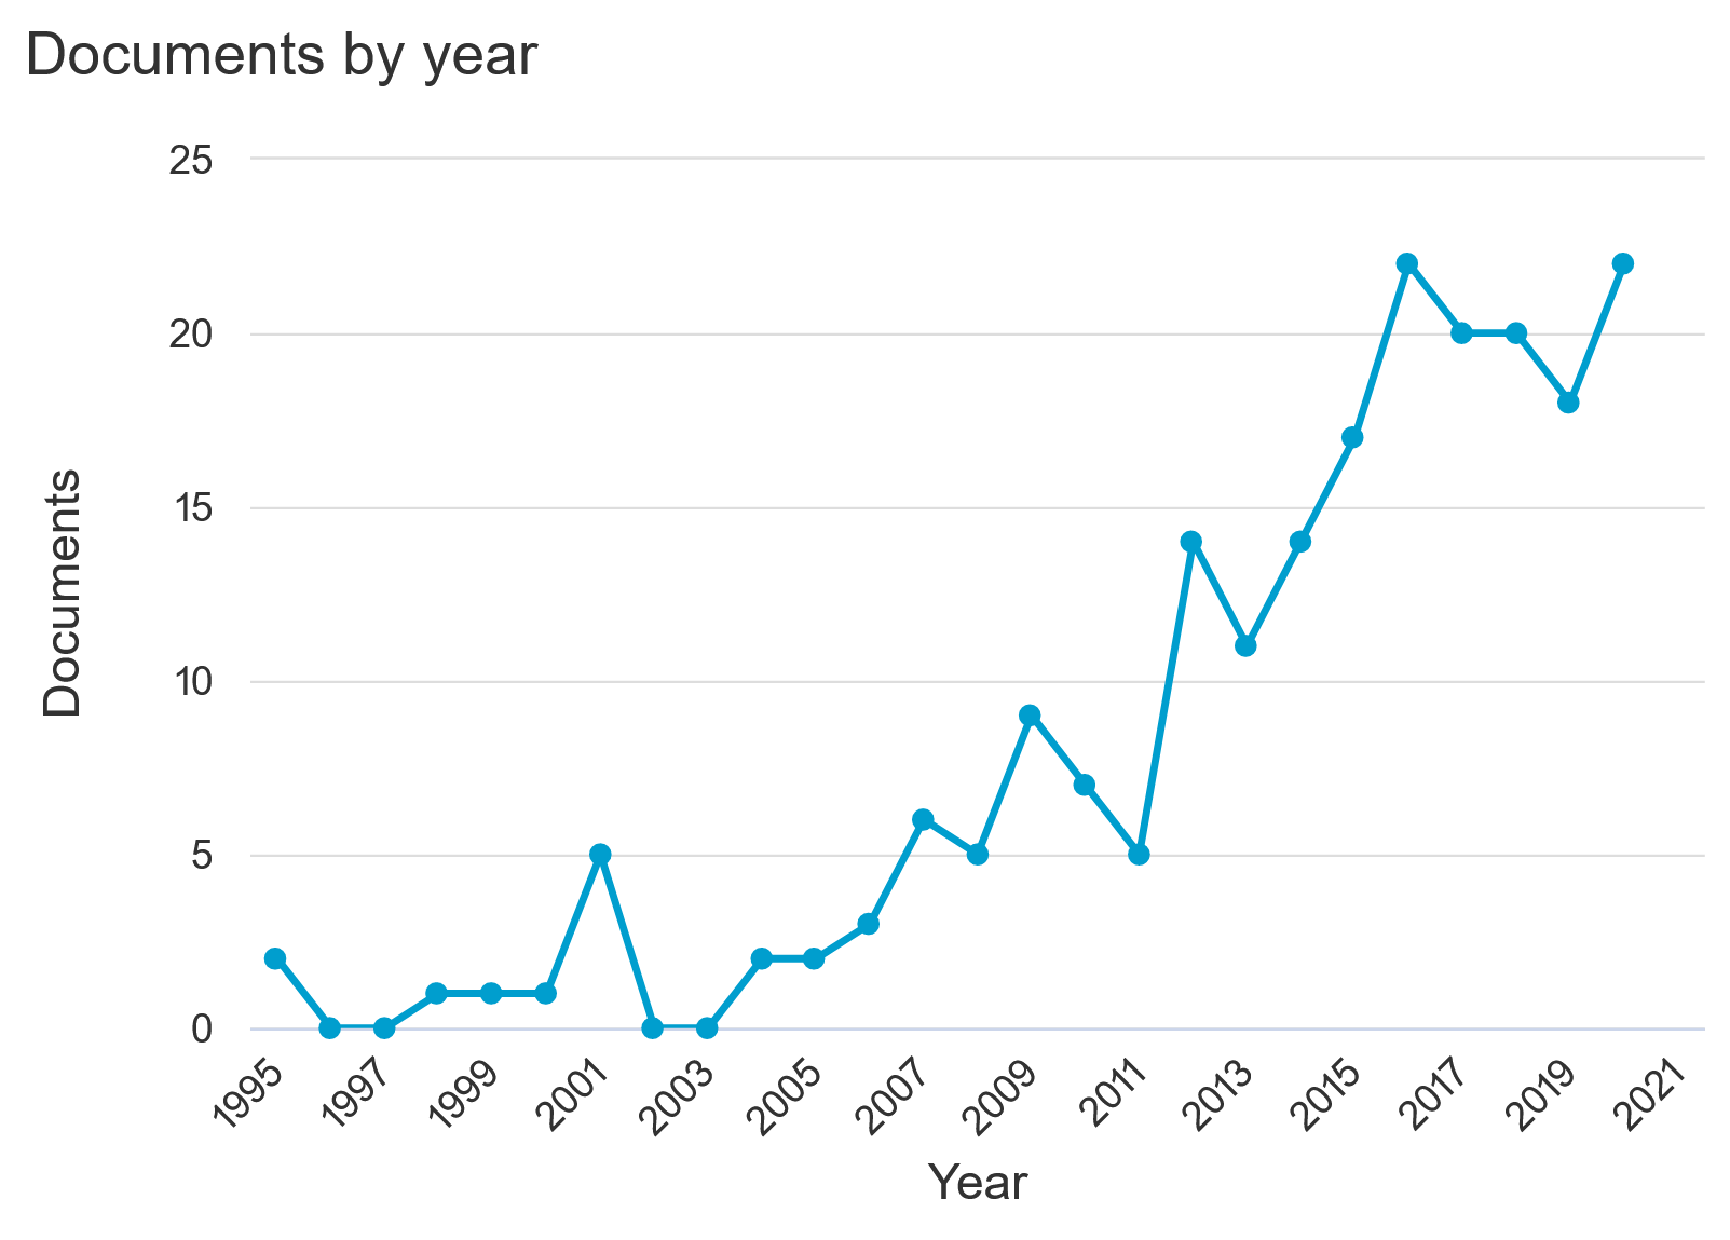
\includegraphics[width=\textwidth]{figures/chap-2/business-needs-hist.pdf}
    \caption{Timeline of the volume of contributions per years for information needs of crisis responders. The year 2021 is excluded because the year is not complete at the time of writing.}
    \label{literature:business-needs-hist}
\end{figure}

The overlay of the keywords generated from the articles retrieved (Figure~\ref{literature:business-needs-overlay}) spans from 2010 to 2018.
It reveals two clusters: one centered on medical issues and another centered on information systems.
The medical cluster focuses on staff well-being and, in particular, on psychological aspects.
The other cluster focuses on emergency services and events management information systems.
This last one is more in connection with the objective of this manuscript; the next analysis will be focused on it.

\begin{landscape}
    \begin{figure}[hp]
        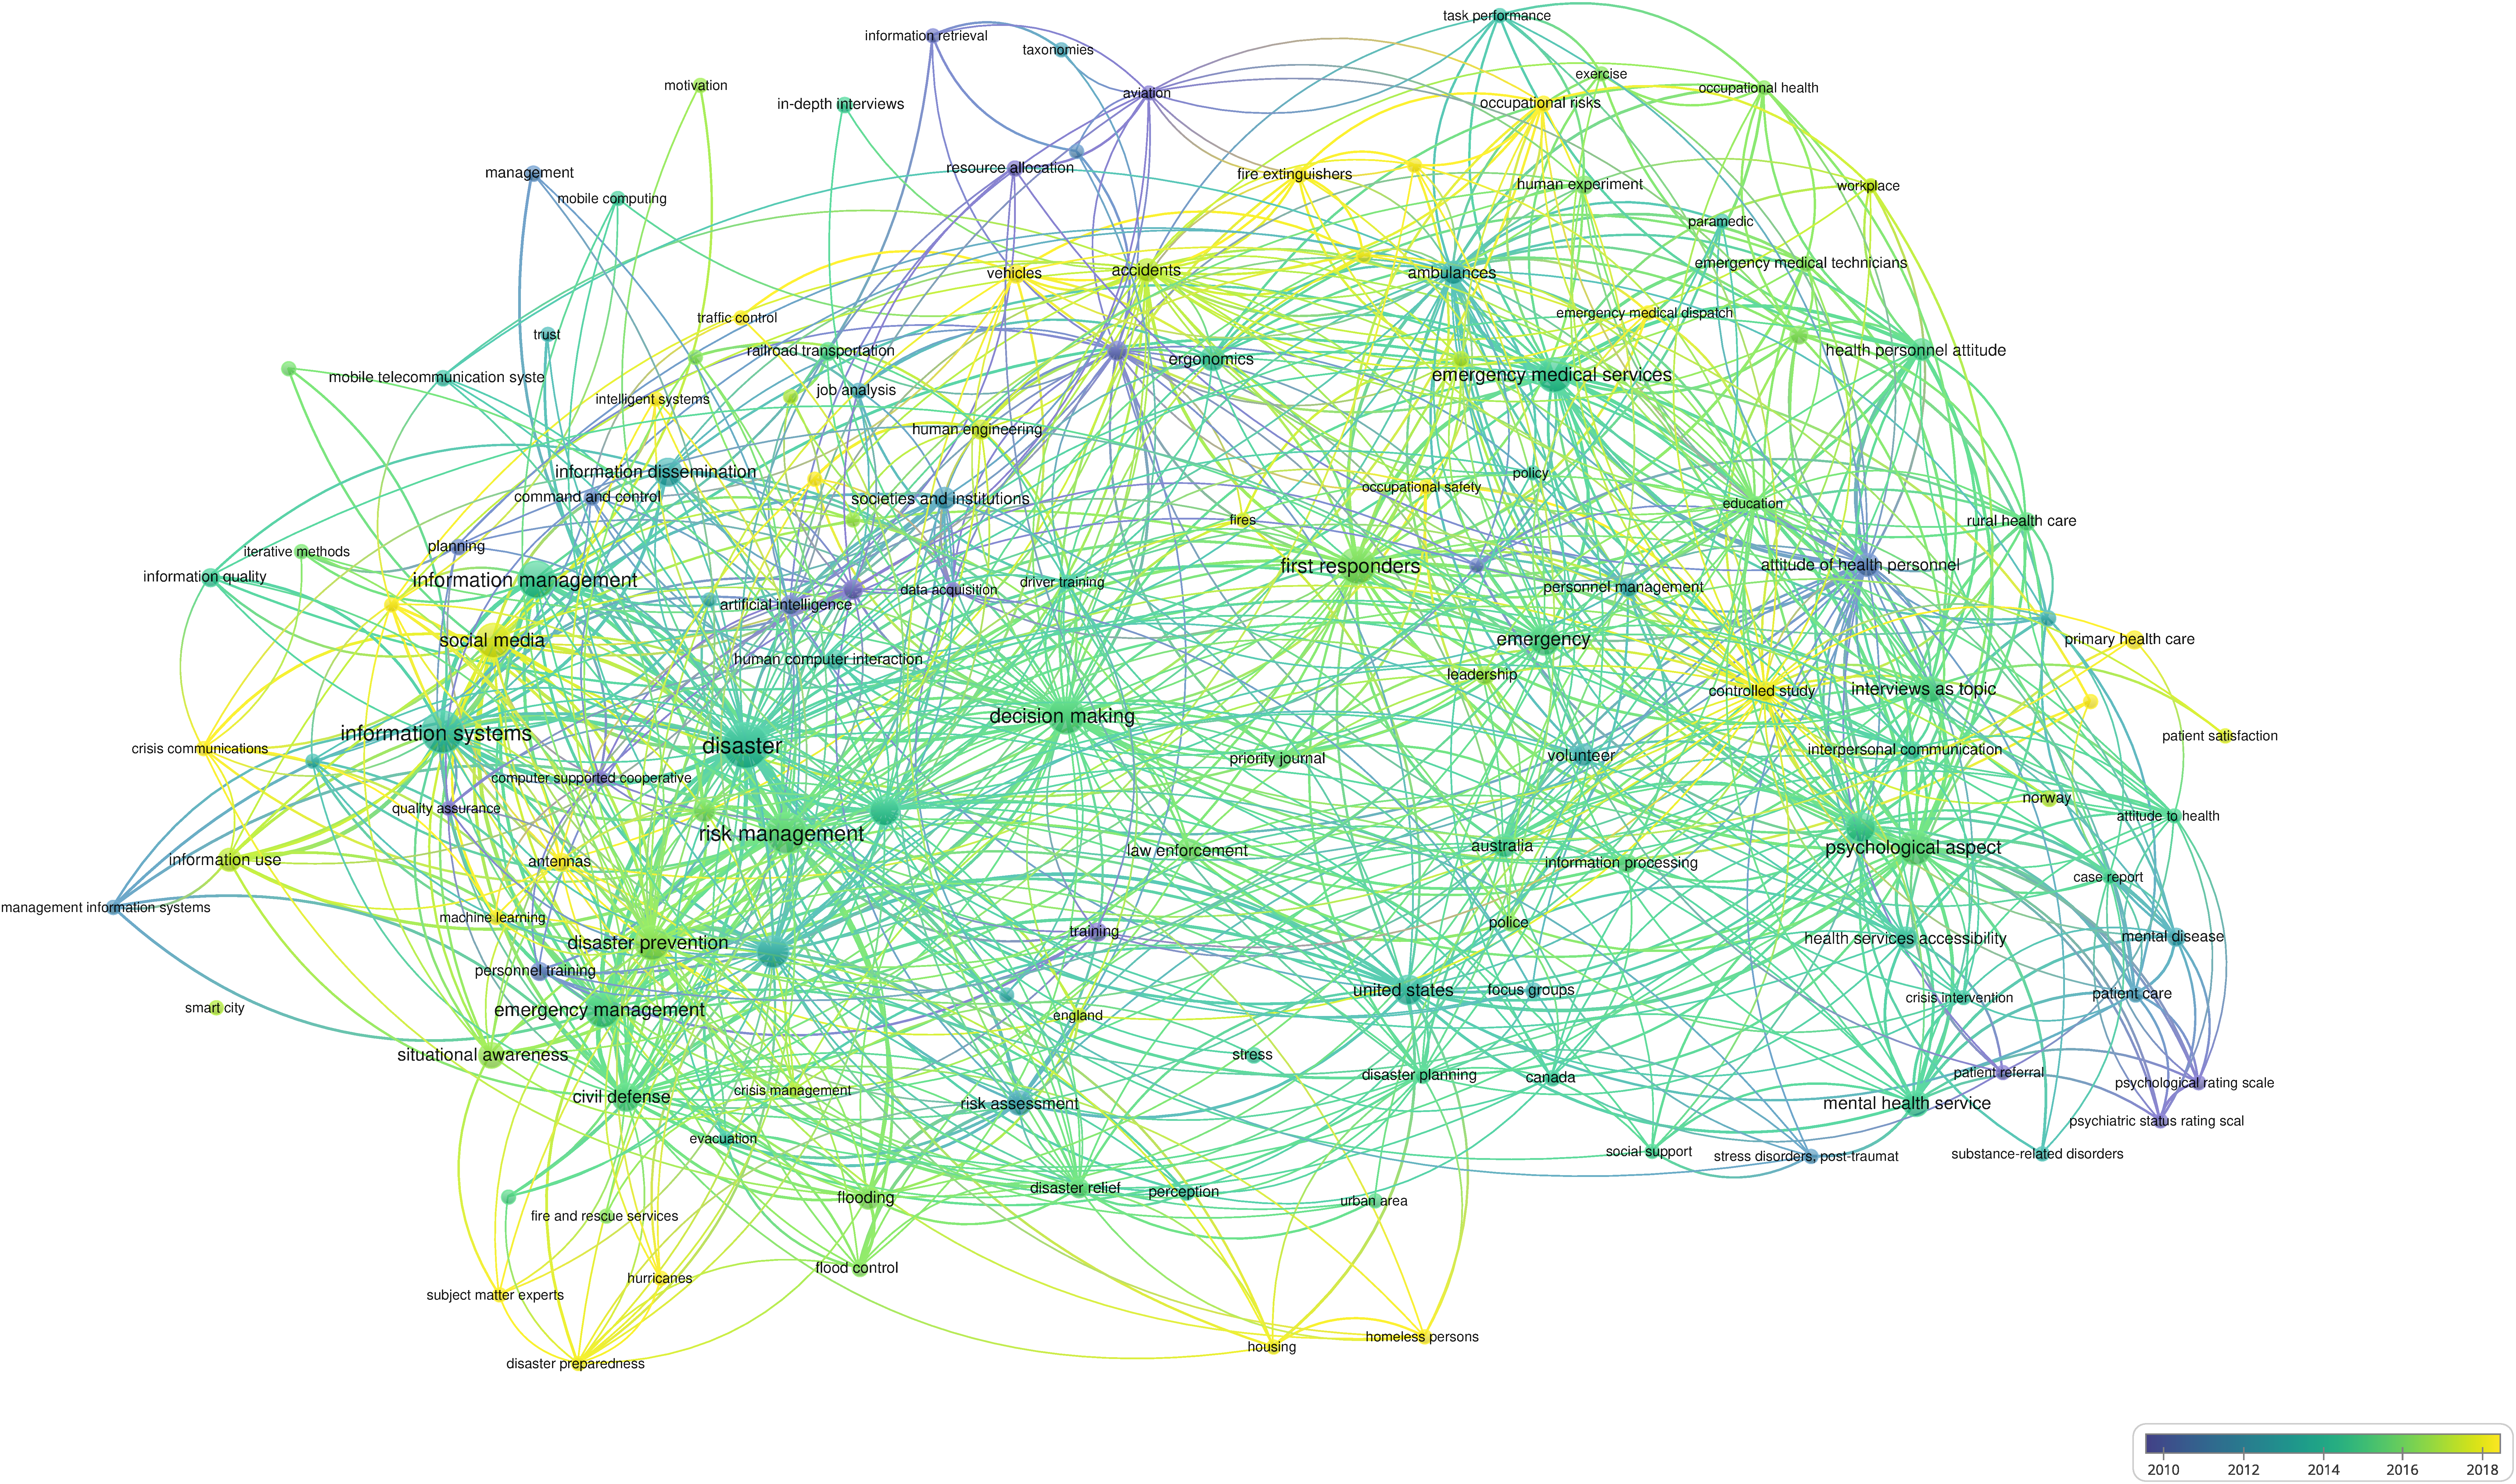
\includegraphics[width=\paperwidth,height=\paperheight,keepaspectratio]{figures/chap-2/business-needs-overlay.pdf}
        \caption{Distribution of keywords with more than 3 occurrences among the articles from the query on information needs of crisis responders.}
        \label{literature:business-needs-overlay}
    \end{figure}
\end{landscape}

The left cluster is composed of the most common keywords used in the fetched articles.
Keywords such as \emph{disaster}, \emph{information systems} and \emph{risk management} (Figure~\ref{literature:business-needs-bar}) are the most prominent ones and seems to be mostly used circa 2014.
Before that period (between 2010 and 2014), the field was primarily focusing on resource or training planning.
But the field took a shift towards data processing to support \emph{decision-making} during emergency events.
The collision with the other domains explored in this chapter seems to happen around 2018, with the use of keywords such as \emph{machine learning}, \emph{social media} or \emph{situational awareness}.

\begin{figure}[thb]
    \centering
    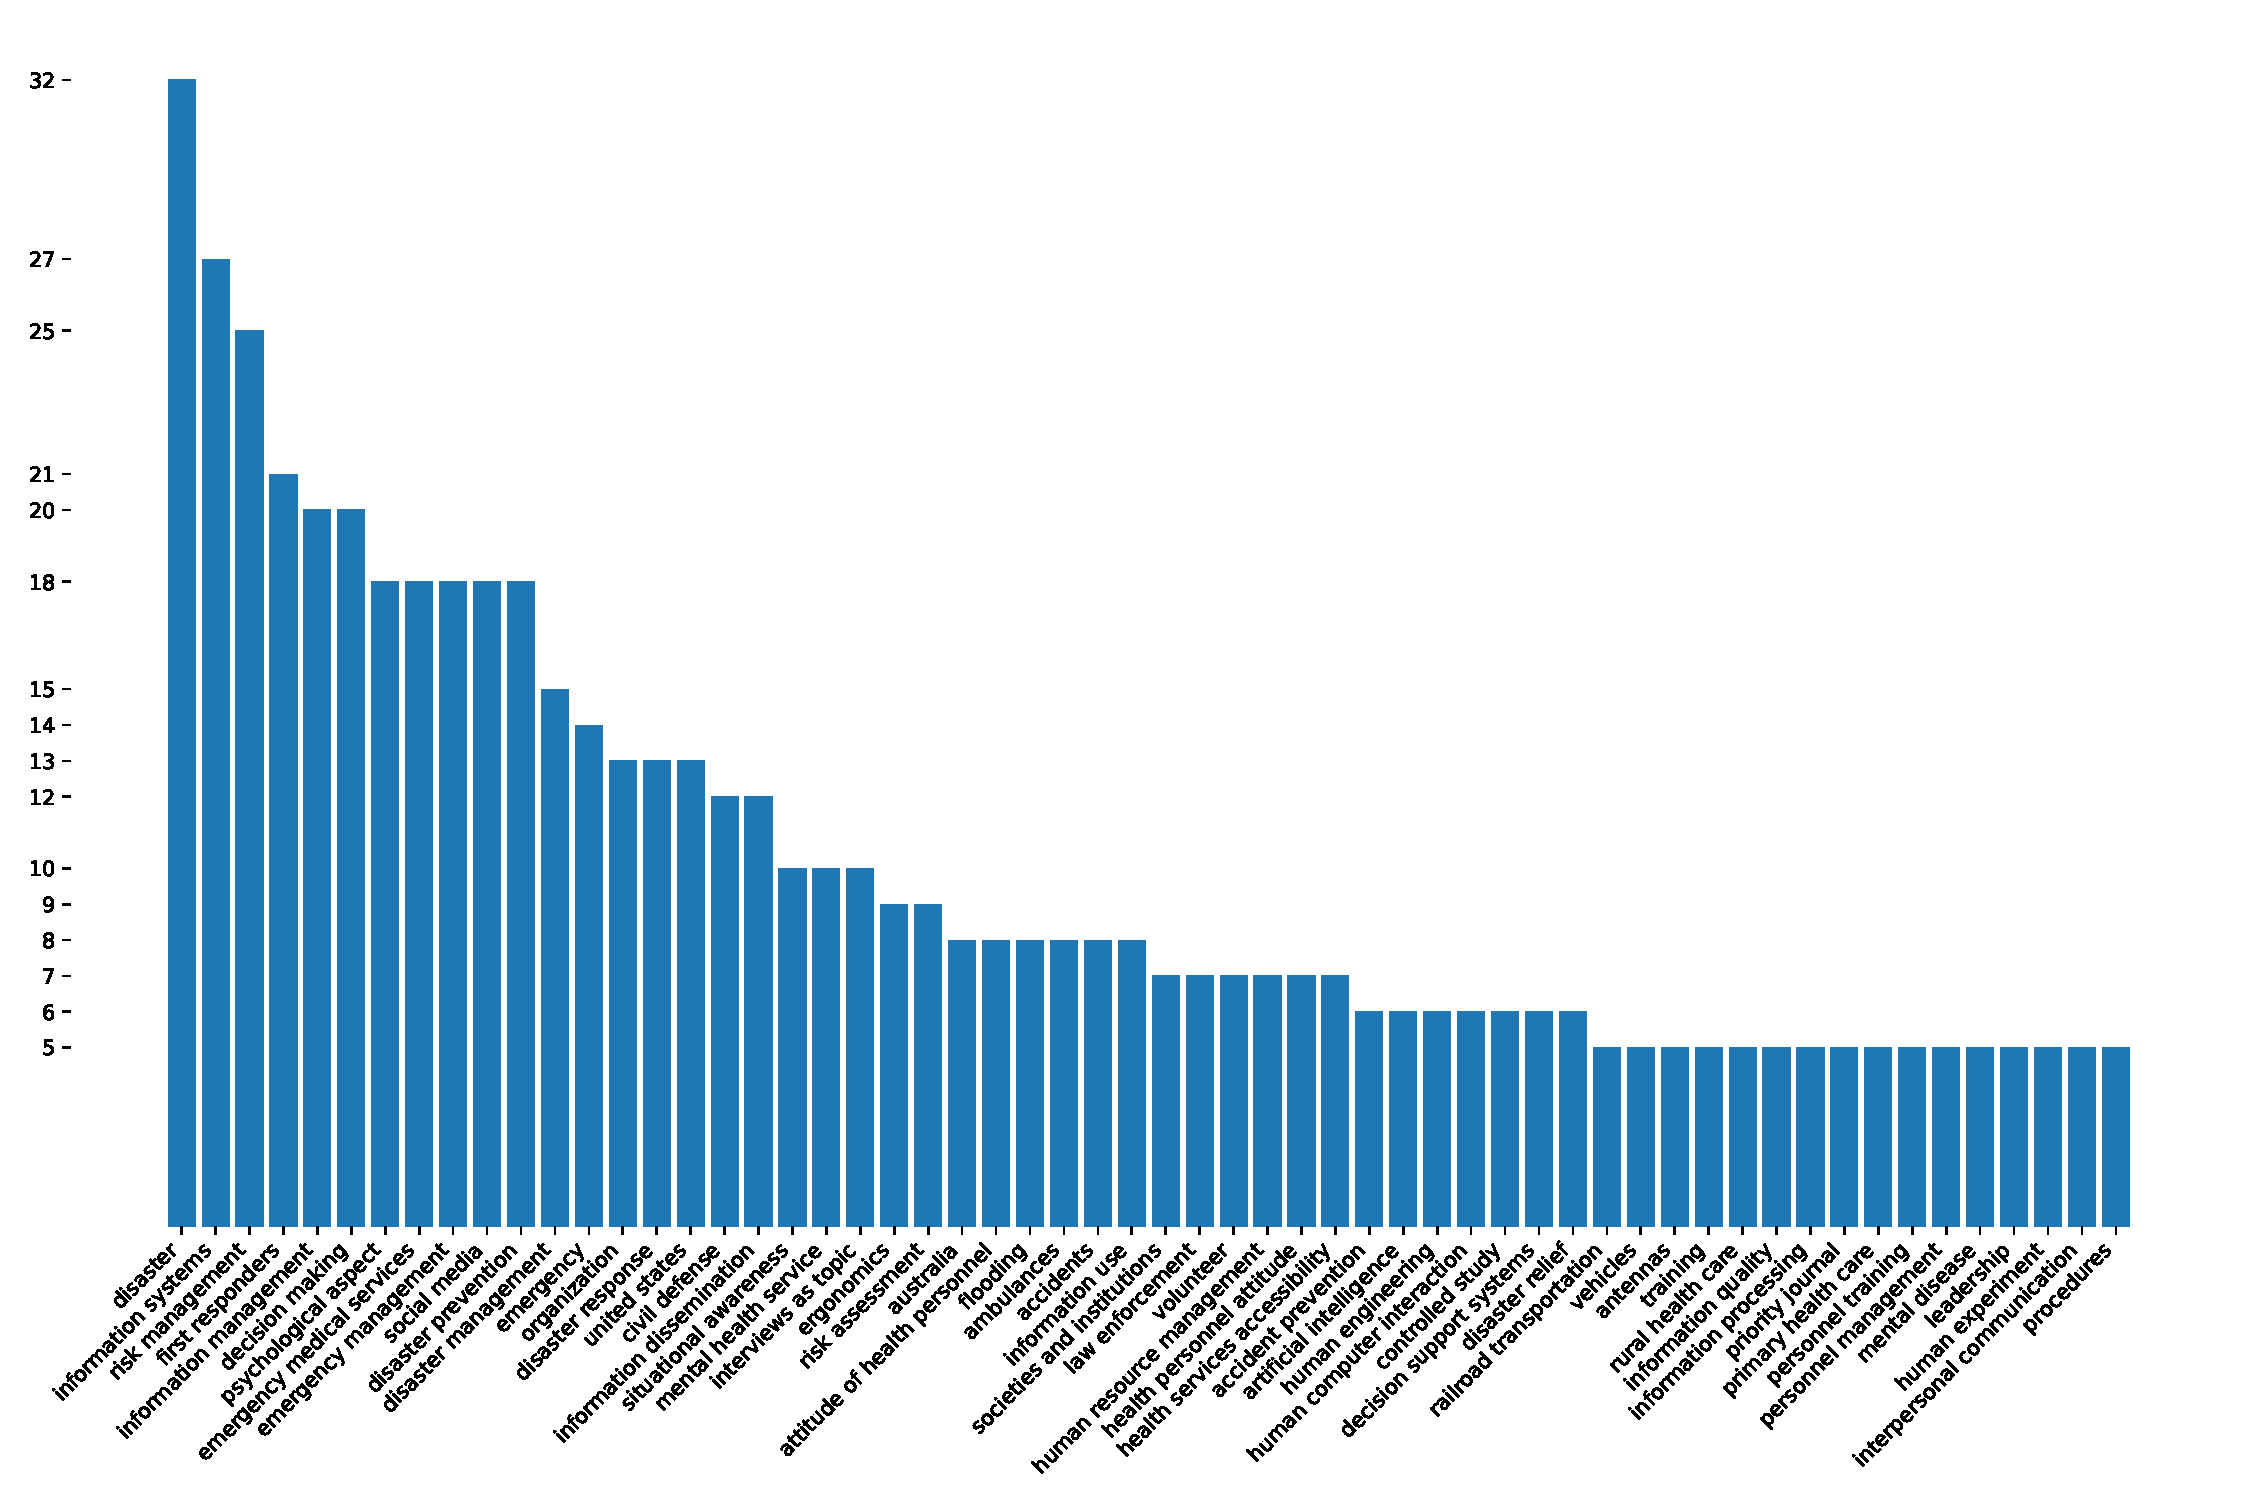
\includegraphics[width=\textwidth]{figures/chap-2/business-needs-bar.pdf}
    \caption{Distribution of keywords with more than 3 occurrences among the articles from the query on information needs of crisis responders.}
    \label{literature:business-needs-bar}
\end{figure}

Table~\ref{table:business-needs-main-articles} provides a summary of the responder's needs identified in the most prominent articles in the field.
Articles were selected if at least 25 citations were published in 2010 or after, are located in the information systems cluster, and are not duplicates.
The articles retrieved provide insights on some of the pain points of emergency organizations.

\begin{table}[bht]
    \centering
    \tabulinesep=1.2mm
    \caption{Articles on informational needs of emergency responders retrieved from the previous request with at least 25 citations.}
    \begin{tabu} to \textwidth {X[1,m]X[3,m]}
        Reference                                                   & Business need identified by the authors.                                                                                                                                                                              \\ [0.5ex]
        \toprule
        \cite{lindellTsunamiPreparednessOregon2010}                 & Tsunami training                                                                                                                                                                                                      \\
        \cite{aloudatRegulationUbiquitousMobile2011}                & Communication to the public                                                                                                                                                                                           \\
        \cite{berlinWhyCollaborationMinimised2011}                  & Collaboration between the different actors                                                                                                                                                                            \\
        \cite{parkerSurfaceWaterFlood2011}                          & Create conversations between unusual actors during the preparation phase                                                                                                                                              \\
        \cite{yangDesignPrinciplesIntegrated2012}                   & Increase situation awareness, Identify key information~\footnote{(hazard environment, information concerning the responder workforce, information on evolving safety issues, and information about safety equipment)} \\
        \cite{tapiaTrustworthyTweetDeeper2013}                      & Accounting for informal sources of data (such as social media)                                                                                                                                                        \\
        \cite{cobbDesigningDelugeUnderstanding2014}                 & Big data processing methods adapted to social media data                                                                                                                                                              \\
        \cite{cabreraaguileraModellingPerformanceVariabilities2016} & Oil spill preparation                                                                                                                                                                                                 \\
        \bottomrule
    \end{tabu}
    \label{table:business-needs-main-articles}
\end{table}

Some studies are event-specific due to a governmental request or a gap in the emergency preparation cover.
\textcite{lindellTsunamiPreparednessOregon2010} is interested in tsunamis management on the US east coast and \textcite{cabreraaguileraModellingPerformanceVariabilities2016} tackle oil spill.
Neither study addresses any particular point in managing this type of event.
Instead, they implement the entire crisis management cycle for these events, which were not considered until their work.
Unfortunately, no specific information needed for decision-makers emerges.

On the other hand, others articles are most focused on the specific needs of emergency organizations.
Collaboration, information sharing and joint preparation exercises are one of the concerns raised \parencite{berlinWhyCollaborationMinimised2011,parkerSurfaceWaterFlood2011}.
The increasing complexity of crisis events asks for a broader range of skills.
As no organization can possess all the required skills simultaneously, other actors must be involved.
Crisis management organizations acknowledge that an unexpected collaboration between actors yields poor outcomes during the response.
Thus, exercises and discussions are critical during the preparation phase, and an adequate means of communication between the actors during the response are needs identified by the studies.

\textcite{yangDesignPrinciplesIntegrated2012} highlight an interesting and well-mentioned need for crisis response: situation awareness.
Situation awareness corresponds to the representation of the state of the environment that surrounds the emergency response organization during an event.
This representation directly guides decision-making.
Consequently, it is critical to build the best and most accurate representation possible at the event's start.
In there are articles, \citeauthor{yangDesignPrinciplesIntegrated2012} emphasize 4 critical pieces of information for situational awareness:

\begin{enumerate}
    \item Environmental conditions such as the building infrastructure, number of occupants, and the exact location of any hazards;
    \item Information on the response participants such as who is involved in the response, what skills they could offer, and what resources they bring to the scene;
    \item The status of any casualties, the accident location, cause, and severity; and
    \item The available resources, including equipment and food.
\end{enumerate}

As per the authors, "timeliness, accuracy, and completeness are the critical dynamic attributes of these four categories of information."
The next chapter (chapter three) will dive deeper into this concept.

The issue with building an accurate situation awareness is the need for information.
With the disruption of regular communication and information channels, decision-makers are shrouded in darkness.
According to \textcite{tapiaTrustworthyTweetDeeper2013,cobbDesigningDelugeUnderstanding2014}, some emergency centers acknowledge the benefit of social media as a potential information source.
However, the issue identified is the lack of tools and methods, similar to those built for calls for social media.

Finally, the last need identified among the extracted items is communication to the public.
\textcite{aloudatRegulationUbiquitousMobile2011} insist on the potential yielded by modern communication means such as cell phones and social media to share information with the public during an event.
People are not always close to a radio or a TV.
Hence, they often miss critical messages during fast-moving events (floods, fires, etc.), resulting in casualties.
On the other hand, (almost literally) most of the population carry a cellphone nowadays, and the critical messages could be distributed faster and with a better viewing rate than traditional methods.
Text messages or notifications from social media could be more effective communication channels that emergency response teams should use.

\subsection{Gathering information on social media?}
The previous two subsections focused on (i) the representations proposed to describe crises and (ii) the challenges organizations face in charge of crisis management.
The overview of these aspects has remained relatively general.
This sub-section, therefore, proposes to refocus the previous analyses on the articles that specifically mention social media.
It also provides insights on the initial research question: What information can be obtained from social media relevant to decision-makers in crisis response?

The keywords "social media" and "Twitter" have been added to the previous queries to refocus on social media.
In the case of the query on crisis models, 18 articles mention social media among 205 initial documents.
The following presents the different information that authors seek from social media.
Thus, ten of the 18 articles do not specify what information they hope to collect but only mention social media as a potential source.
The findings from the remaining articles are summarized in Table~\ref{table:information-model-social-media}.
% \parencite{pobletCrowdsourcingRolesMethods2018,kemavuthanonIntegratedQuestionansweringSystem2020b,khzamDomainspecificSoftwareLanguage2018,mossgraberSensorDecisionChain2018,laudyRumorsDetectionSocial2017,hayesCareEthicsResponsible2020}
he table highlights the main information that the authors wish to use to implement the ontologies they propose.
Information about the event, such as its type and effects, is the most common information required.
Victims' information is also mentioned in several studies.
Interestingly, the studies seem to fall into two groups.
In the first group, ontologies are created before retrieving posted messages.
In this group, the authors thus seek to filter the messages that correspond to the ontologies they use \parencite{gaurEmpathiOntologyEmergency2019,moiDesignOntologyUse2016,narayanasamyCrisisDisasterSituations2019b,montarnalAutomatedEmergenceCrisis2017,cocheActionableCollaborativeCommon2019c}.
The second group follows a similar approach but proceeds to the first phase of message collection, whose content feeds the ontology construction.
The ontologies thus obtained are then "closer" to social media by "moving away" from crisis management \parencite{kemavuthanonClassificationSocialMedia2020b,kawtrakulImprovingDisasterResponsiveness2012,leeConstructionEventOntology2013}.

\begin{table}[bht]
    \centering
    \tabulinesep=1.2mm
    \caption{Articles on informational needs of emergency responders retrieved from the previous request with at least 5 citations.}
    \begin{tabu} to \textwidth {X[1,m]X[3,m]}
        Reference                                            & Information authors are looking for from social media                       \\ [0.5ex]
        \toprule
        \textcite{purohitIdentifyingSeekersSuppliers2014}    & Victims' needs and people offering resources.                               \\
        \textcite{gaurEmpathiOntologyEmergency2019}          & Location, Event type and impact, Victims, Resource, Actors involved, Status \\
        \textcite{ghahremanlouGeotaggingTwitterMessages2014} & Geographic location                                                         \\
        \textcite{bhattAssistingCoordinationCrisis2014}      & Victims' needs                                                              \\
        \textcite{zavarellaOntologybasedApproachSocial2014}  & Event type, Event impact, Location, Weapon inolved, Organizations involved  \\
        \textcite{cocheActionableCollaborativeCommon2019c}   & Location, Event type, Weapon involved, Victims                              \\
        \textcite{montarnalAutomatedEmergenceCrisis2017}     & Crisis related messages, Event type, Time of publication                    \\
        \textcite{leeConstructionEventOntology2013}          & User name, Time of publication, Location, Event type                        \\
        \bottomrule
    \end{tabu}
    \label{table:information-model-social-media}
\end{table}

The same methodology is then applied to the needs of crisis management organizations.
Adding the keywords \emph{social media} and \emph{Twitter} indicates that 21 of the 219 articles previously retrieved are related to these topics.
Unlike the studies retrieved in the previous query, these rarely consider categories of social media information.
Table~\ref{table:business-needs-social-media} summarizes the different approaches considered in the main articles.
Among these articles are common interests that can be grouped into three categories.
First, the involvement and consideration of volunteers in crisis management \parencite{smithSocialMediaCitizenled2018,graceCommunityCoordinationAligning2018,nielsenEmbracingIntegratingSpontaneous2019,cobbDesigningDelugeUnderstanding2014}.
Another group of studies focuses on filtering information from social media to reduce the volume of information reaching decision-makers.
The aim is to avoid an information overload that would be detrimental to the conduct of the response \parencite{onealTrainingEmergencyresponseImage2019,norri-sederholmEnsuringInformationFlow2017,moiStrategyProcessingAnalyzing2016,kaufholdMitigatingInformationOverload2020}
Finally, the last group focuses on the veracity of social media content and the information they expose to response organizations.
As such, two of the four publications highlight the usefulness of this content for the response, while the other two call for more caution \parencite{mehtaTrustVerifySocial2017,tapiaTrustworthyTweetDeeper2013,tapiaGoodEnoughGood2014,vangorpJustKeepTweeting2015}.

\begin{table}[bht]
    \centering
    \tabulinesep=1.2mm
    \caption{Articles on informational needs of emergency responders retrieved from the previous request with at least 5 citations.}
    \begin{tabu} to \textwidth {X[1,m]X[3,m]}
        Reference                                             & Approach to information from social media                         \\ [0.5ex]
        \toprule
        \textcite{cobbDesigningDelugeUnderstanding2014}       & People requiring or providing resources                           \\
        \textcite{graceCommunityCoordinationAligning2018}     & Consideration of citizen reports posted on social media           \\
        \textcite{kaufholdMitigatingInformationOverload2020}  & Reducing information overload through social media filtering      \\
        \textcite{mehtaTrustVerifySocial2017}                 & Evaluation of uncertainty of information coming from social media \\
        \textcite{moiStrategyProcessingAnalyzing2016}         & Reducing information overload through social media filtering      \\
        \textcite{nielsenEmbracingIntegratingSpontaneous2019} & Considering volunteers in crisis management                       \\
        \textcite{norri-sederholmEnsuringInformationFlow2017} & Importance of information flow to reduce information overload     \\
        \textcite{onealTrainingEmergencyresponseImage2019}    & Image classification to detect rescuers and rescuees              \\
        \textcite{smithSocialMediaCitizenled2018}             & Social media use of volunteers during disaster                    \\
        \textcite{tapiaGoodEnoughGood2014}                    & Evaluation of uncertainty of information coming from social media \\
        \textcite{tapiaTrustworthyTweetDeeper2013}            & Evaluation of the usefulness of social media content              \\
        \textcite{vangorpJustKeepTweeting2015}                & Evaluation of the usefulness of social media content              \\
        \bottomrule
    \end{tabu}
    \label{table:business-needs-social-media}
\end{table}

This section has gone through different aspects of the research question: \emph{What can decision-relevant information from social media be processed automatically?}
The first two sections have explored information processing in crisis management globally along two axes.
The first axis is the crisis models designed and proposed by computer sciences.
We have seen that a great diversity of models have been proposed.
This diversity mainly results from the granularity or scale adopted by the authors or the type of disaster studied.
The second axis has adopted the point of view of the social sciences on these issues.
The latter has allowed us to understand the numerous issues of emergency organizations in managing their information.
The final part of this section focused on the studies from both approaches that considered social media as a source of information.
In this context, most of the research from the computer science community focused on implementing different ontologies proposed.
The teams that presented the information that was attempting to retrieve mostly focused on the following information:

\begin{itemize}
    \item Event type
    \item Event consequences
    \item Victims status
    \item Victims needs
    \item Location
\end{itemize}

On the other hand, social studies are less interested in what information is processed but rather in how it is processed.
Three main topics appear from the set of studies highlighted in this part.
First, consider physical and digital volunteers in crisis response and include them in the official process.
Secondly, managing the flow of information to avoid information overload.
This research group is directly aligned with the views of the computer science domain.
The final research group focuses on assessing the value of social media information for crisis management.
Interestingly, each axis has a different approach to managing social media information during crisis response.
The first axis took a top-down approach by thinking about representations that are then confronted with reality.
The second axis took the other direction, with a bottom-up approach, where authors interview practitioners to identify points of interest.
This section highlighted the need and previous attempts to automate the collection and management involved in crisis management.
Also, it showed that social media are a source of valuable information that requires appropriate means of processing.
Thus, the following section discusses existing means of identifying and mining information from social media.

\section{NLP methods for information extraction from social media data}
The first chapter presented the Natural Language Processing (NLP) domain.
Through the development of this domain, many tools, algorithms, and methods have been developed to process textual data.
With the emergence of social media, a new source of textual data appeared, and with it, its own challenges.
This chapter explores the following research question: \emph{How can this information be obtained in the context of crisis informatics?}
Social media data are used as a data source in various use cases.
This section is broken down into two parts, and it aims to explore two directions.
First, for which applications is NLP used on social media data?
Secondly, what are the methods used to extract information from social media?
Each question is treated in a sub-section.
To explored these two direction the following request is run:

\begin{table}[bht]
    \centering
    \tabulinesep=1.2mm
    \caption{Overview of the bibliographic request related to challenges in crisis management.}
    \begin{tabu} to \textwidth {X[0.5,r]X[1,m]X[1,m]}
        Type of request & Keywords                                                            & Explaination                                                                      \\ [0.5ex]
        \toprule
        SUBJAREA        & \textit{comp}                                                       & Articles in either Computer Science, Social Sciences of Decision Sciences domains \\
        TITLE-ABS-KEY   & \textit{natural language processing} OR \textit{information mining} & Articles focus on natural language processing or information mining               \\
        TITLE-ABS-KEY   & \textit{social media} OR \textit{Twitter}                           & To process social media data                                                      \\
        TITLE-ABS-KEY   & \textit{survey}                                                     & Only surveys are considered in this section                                       \\
        EXCLUDE-DOCTYPE & \textit{re} OR \textit{cr}                                          & Reviews and conference tracks introductions are excluded                          \\
        \bottomrule
    \end{tabu}
    \label{table:nlp-challenges}
\end{table}

This section will only consider surveys published in the domain.
This choice is made to filter the numerous publications in this area.
Without this constraint, the request returns 4231 documents.
This large volume of publications, which reflects the popularity of the field, makes it challenging to analyze the field's evolution.
However, restricting the results in this way should not prevent reporting on trends in the field.
The request presented in Table~\ref{table:nlp-challenges} returns 217 surveys, published between 2011 and 2021 (Figure~\ref{literature:nlp-hist}).
While being a relatively recent research venue, the interest in NLP uses on social media data has increased over the years.

\begin{figure}[thb]
    \centering
    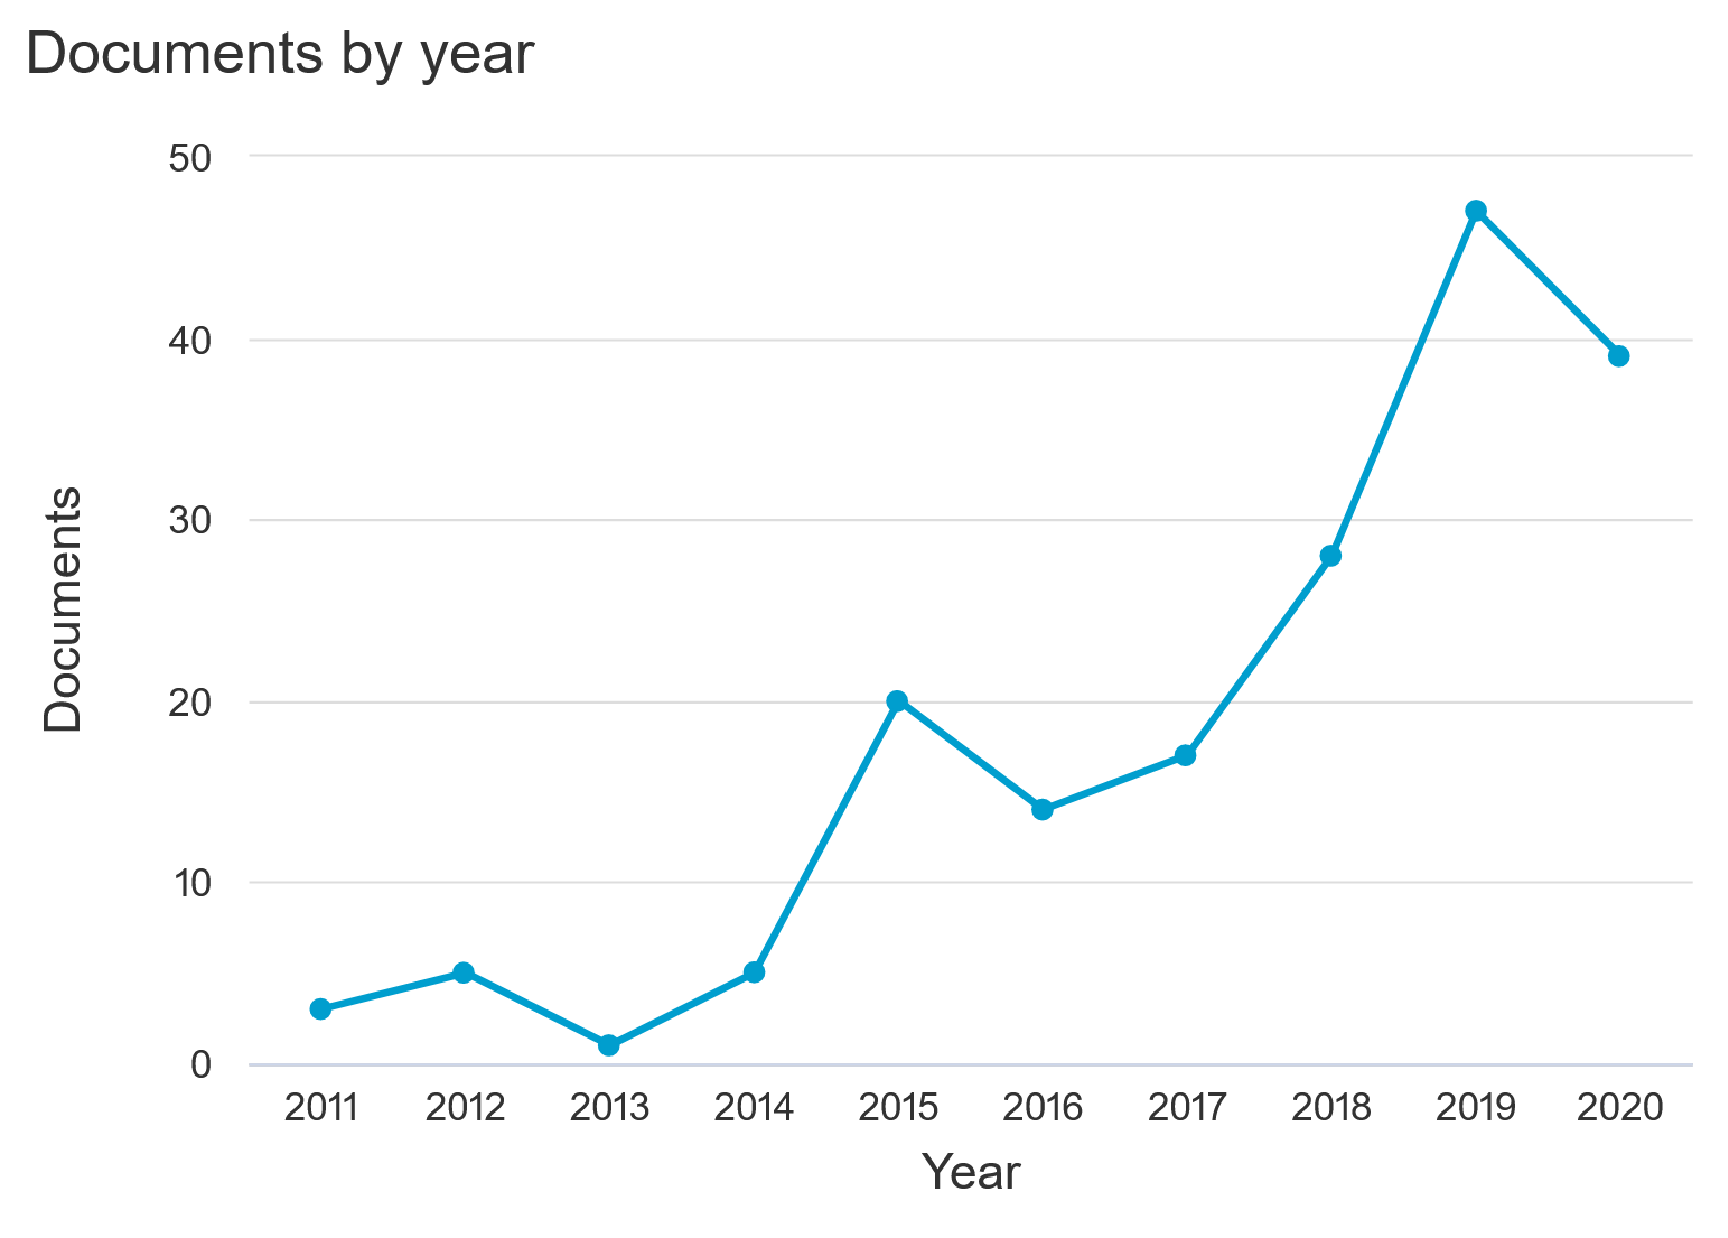
\includegraphics[width=\textwidth]{figures/chap-2/nlp-hist.pdf}
    \caption{Timeline of the volume of contributions per years for the application of NLP methods to social media data. The year 2021 is excluded because the year is not complete at the time of writing.}
    \label{literature:nlp-hist}
\end{figure}

The surveys retrieved appear as a single cluster (Figure~\ref{literature:nlp-overlay}).
This overlay was created by aggregating synonyms, removing the keywords from the query, and some keywords with a low value for our study ("state of the art, large amounts, codes (symbols), research questions, text").
Despite the field's youth, its evolution is swift, both in applications and methods used.
Circa 2011, the field was centered around epidemiological applications and statistical analyses.
From this point on, a kaleidoscope of applications and methods was used.
They are detailed in the following two subsections.

\begin{landscape}
    \begin{figure}[hp]
        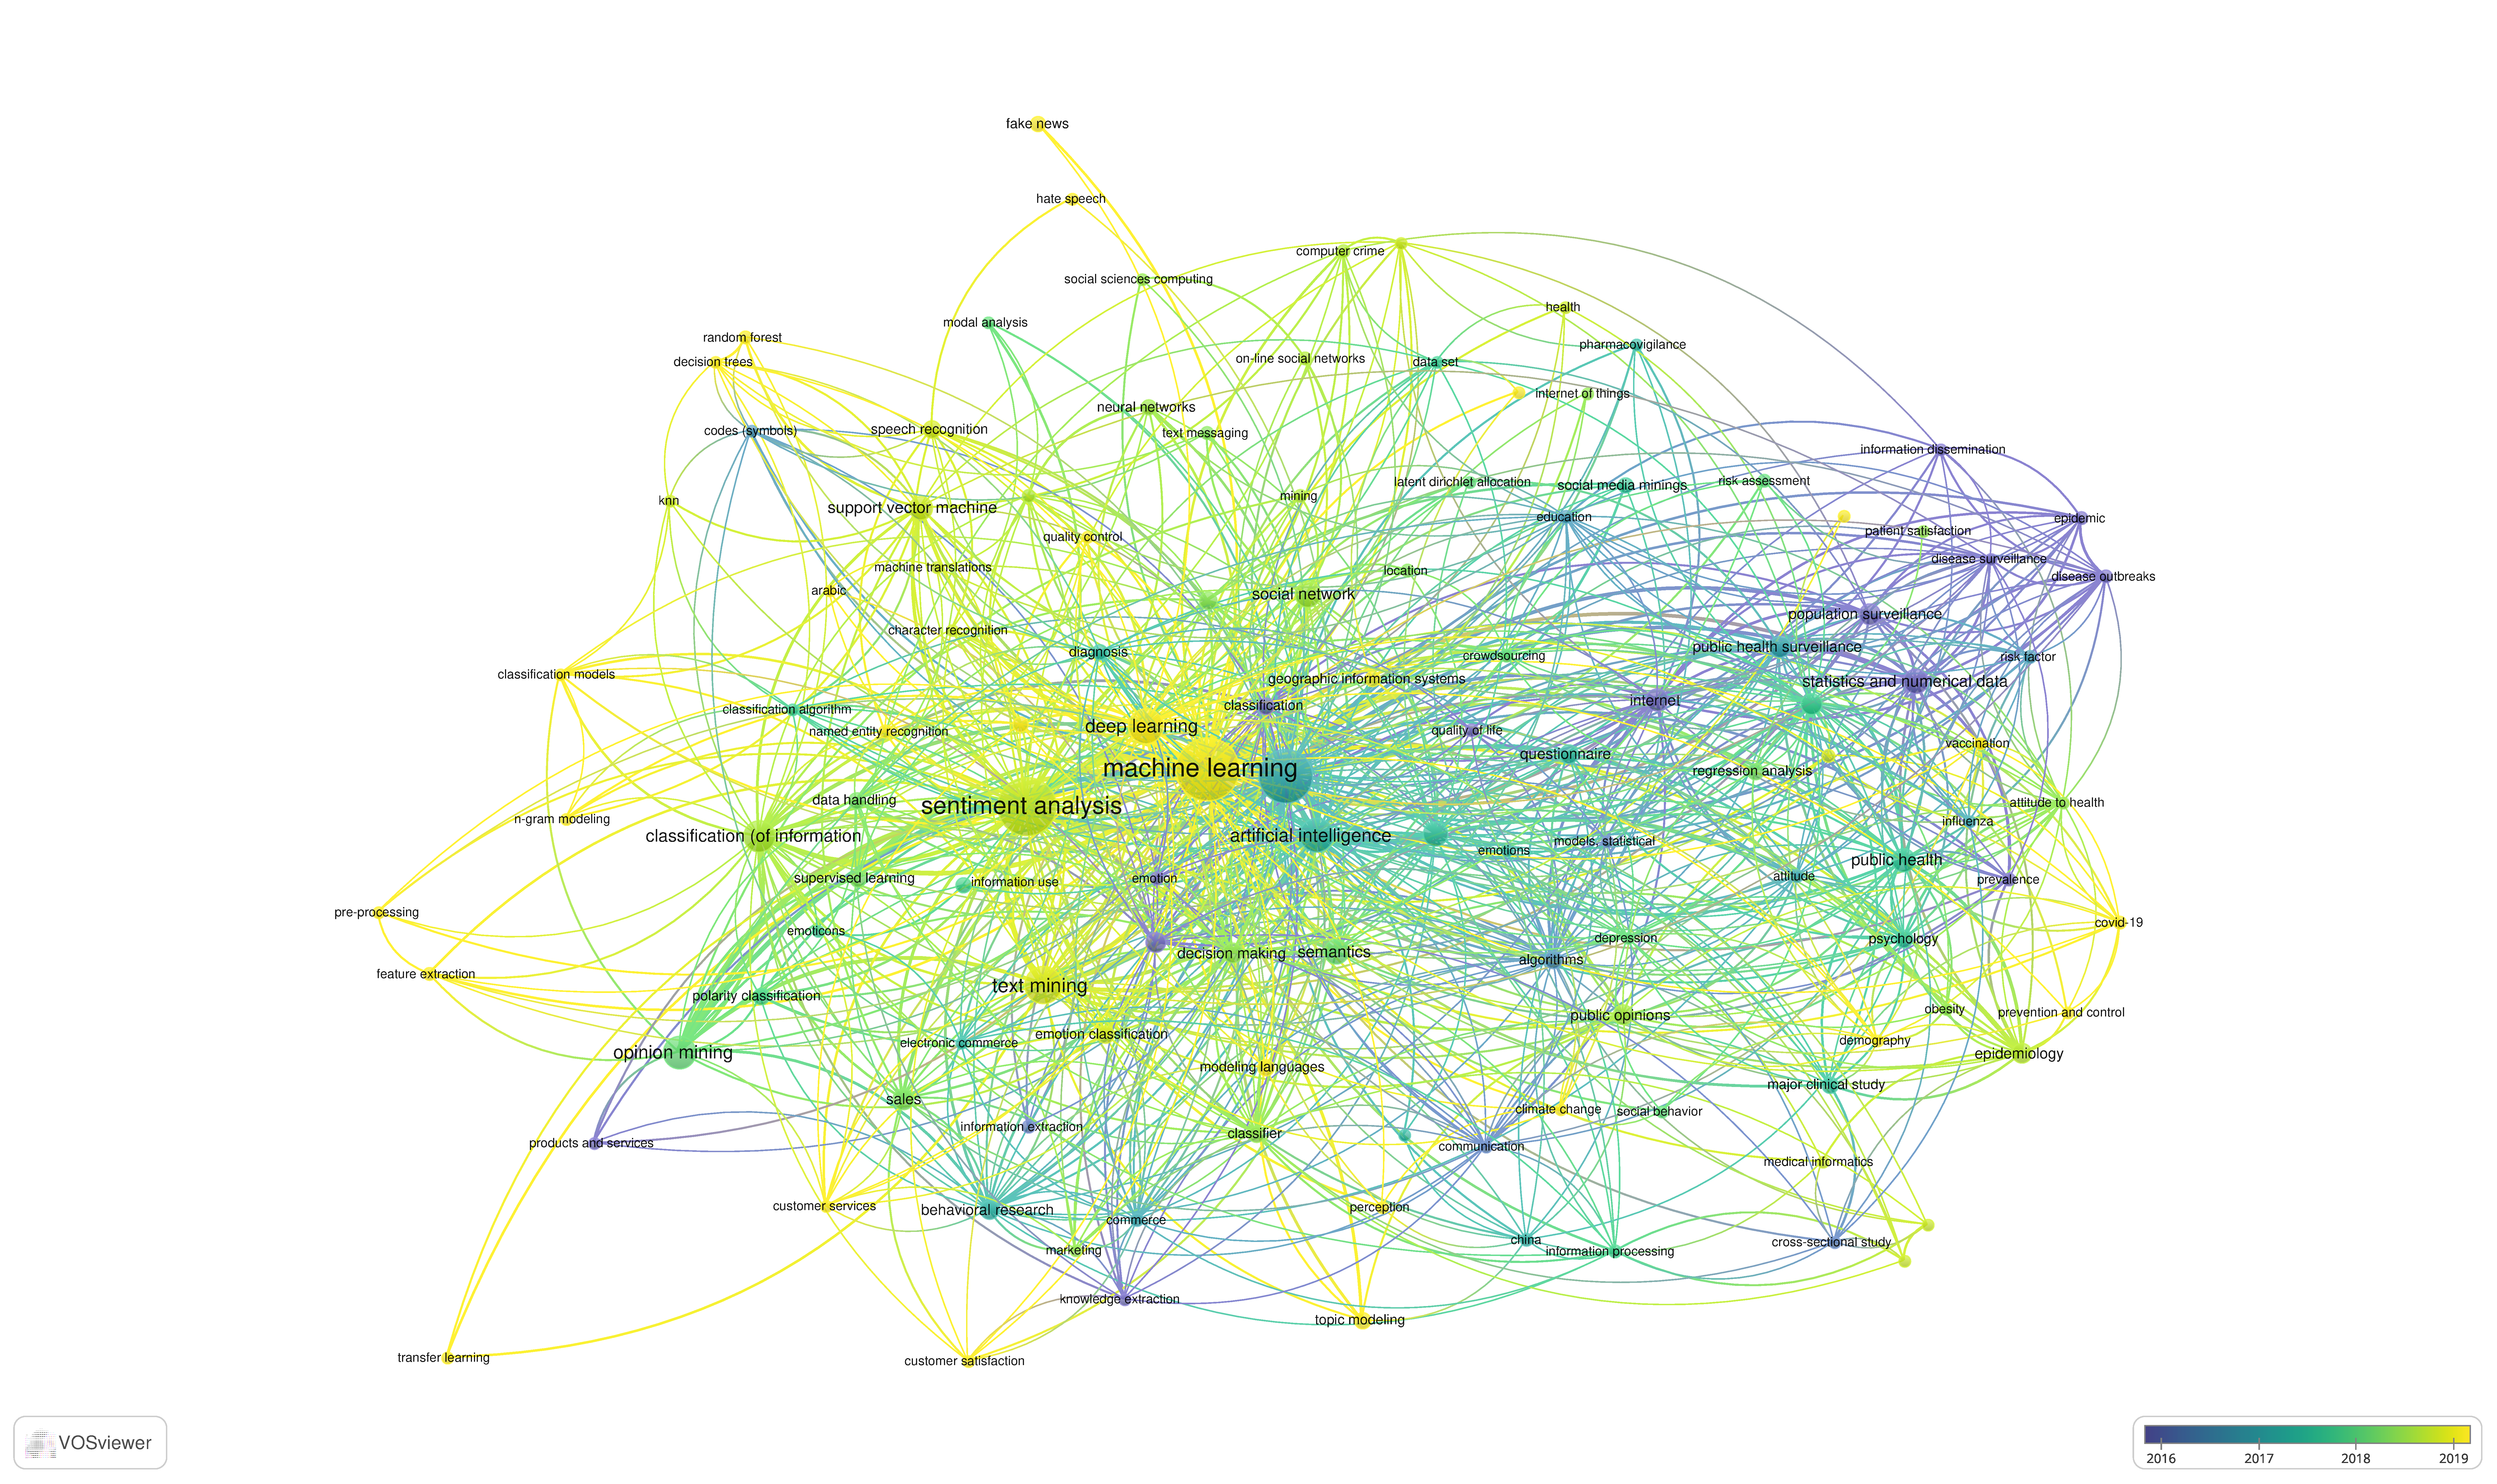
\includegraphics[width=\paperwidth,height=\paperheight,keepaspectratio]{figures/chap-2/nlp-overlay.pdf}
        \caption{Distribution of keywords with more than 3 occurrences among the articles from the query on NLP applied on social media data.}
        \label{literature:nlp-overlay}
    \end{figure}
\end{landscape}

However, some keywords trends have been more prominent during these years than others.
On the application side, \emph{sentiment analyses} is by far the most studied application (73 mentions of this keyword) (Figure~\ref{literature:nlp-bar}).
Mining applications are second with \emph{data mining} (mentioned 61 times), \emph{text mining} (30 times) and \emph{opinion mining} (mentioned 21 times).
On the method side, \emph{artificial intelligence} (mentioned 25 times), and especially \emph{machine learning} (85 times, almost half surveys) methods (such as shown with the appearance of \emph{deep learning}) are heavily mentioned as well in the surveys.
These methods illustrate the importance of the applications of machine learning methods in natural language processing.

\begin{figure}[thb]
    \centering
    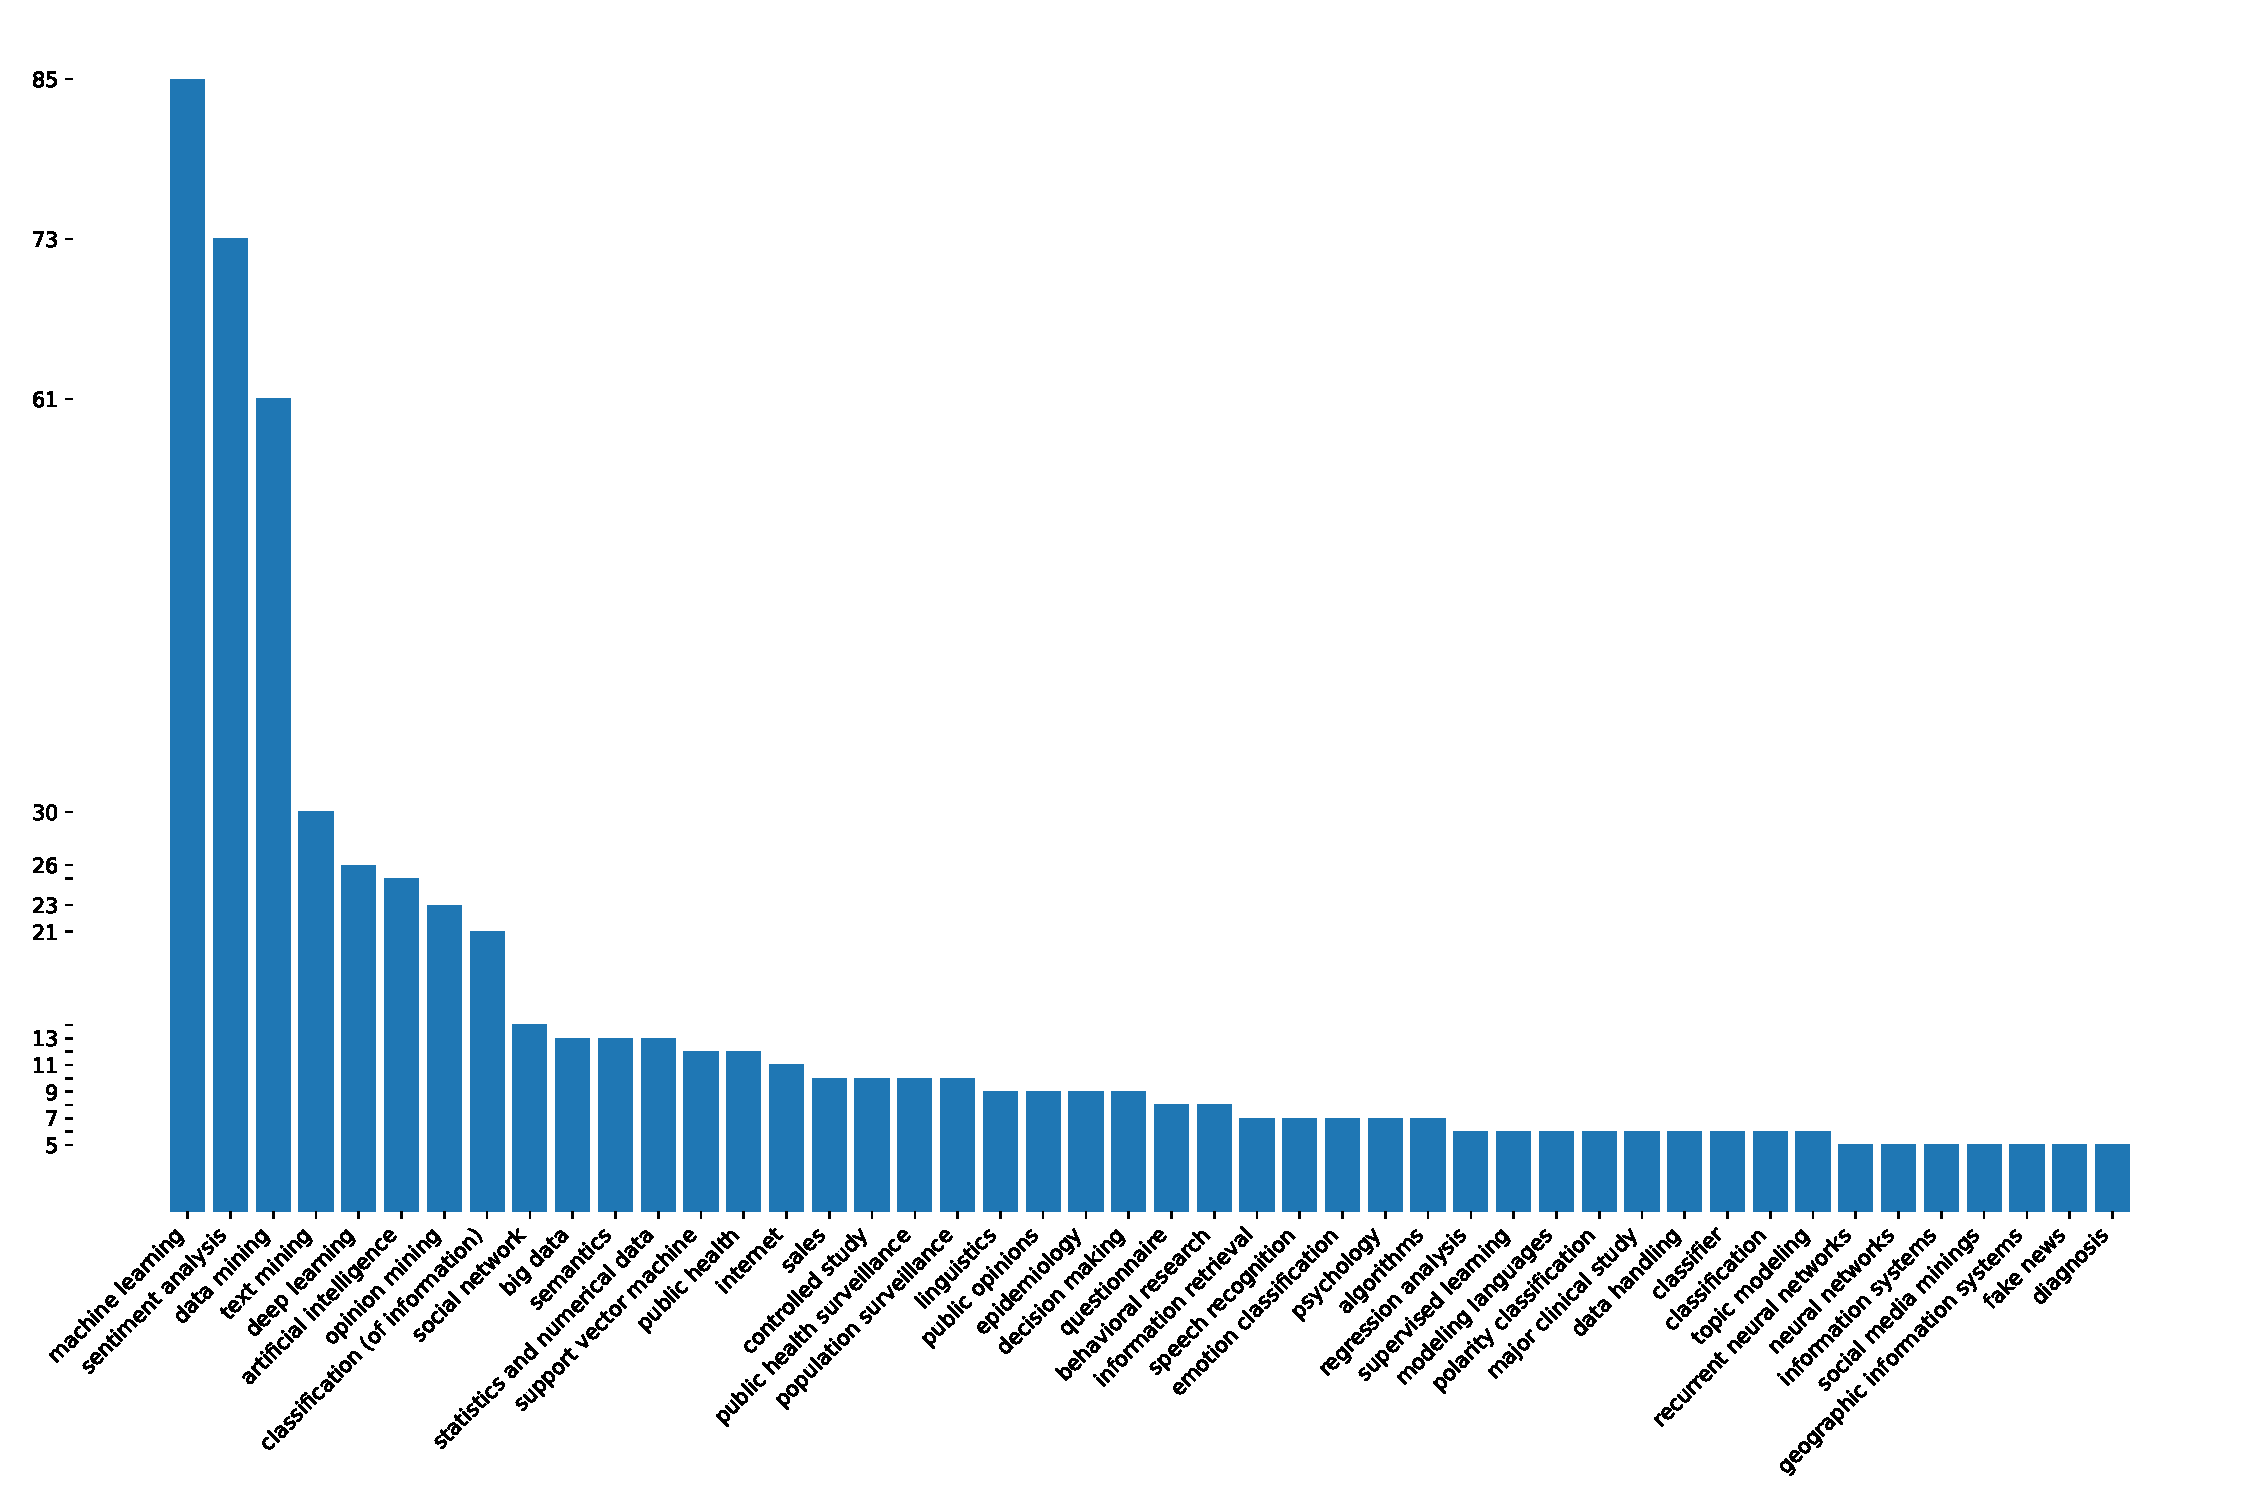
\includegraphics[width=\textwidth]{figures/chap-2/nlp-bar.pdf}
    \caption{Distribution of keywords with more than 4 occurrences among the articles from the query on NLP applied on social media data.}
    \label{literature:nlp-bar}
\end{figure}

Table~\ref{table:nlp-main-articles} presents the main surveys, their focus, and the associated field of application.
Specifically, 27 surveys cited more than 25 times appear.
These 27 documents are divided into seven topics:

\begin{itemize}
    \item Sentiment analysis
    \item Epidemiology
    \item Health
    \item Text mining
    \item Social Network
    \item Uncertainty
\end{itemize}

Nine surveys compose the sentiment analysis topic \parencite{yadavSentimentAnalysisUsing2020,hemmatianSurveyClassificationTechniques2019,chaturvediDistinguishingFactsOpinions2018,raviSurveyOpinionMining2015,chamlertwatDiscoveringConsumerInsight2012,liuSurveyOpinionMining2012,jiangAssessmentOnlinePublic2016,hawkinsMeasuringPatientperceivedQuality2016}.
It is a well-discussed topic as surveys span from 2012 to 2020.
The main objective of sentiment analysis is usually to detect if a message is positive or negative about the topic of the message.
Emotion detection is the next step after sentiment analysis.
It can be more challenging, as it is required to classify text messages to a large variety of emotions that are notably hard to capture \parencite{sailunazEmotionDetectionText2018,poriaReviewAffectiveComputing2017}.
These two subjects make up almost half of the volume of publications highlighted.
Eight articles are related to medical topics.
Four are using social media to study the spread of diseases among the population such as influenza \parencite{kagasheEnhancingSeasonalInfluenza2017,santillanaCombiningSearchSocial2015}, Ebola \parencite{odlumWhatCanWe2015}, and opioids \parencite{charyEpidemiologyTweetsEstimating2017}.
Three others survey the public behavior related to depression \parencite{yazdavarSemiSupervisedApproachMonitoring2017,khzamDomainspecificSoftwareLanguage2018} and to inflammatory disease \parencite{martinezPatientUnderstandingRisks2017}.
Four surveys identify the various approaches available and used in different contexts.
\textcite{salloumSurveyTextMining2017} review different existing methods, while \textcite{paulSocialMediaMining2016} focuses on applications to public health, \textcite{wangSocialMediaSensor2015} on air quality and \textcite{collierUncoveringTextMining2012} epidemiology.
NLP applied to social media also provides valuable insights on social media themselves or the social network of its users.
Three surveys are focusing on these aspects, with \textcite{bailCombiningNaturalLanguage2016} studying advocacy groups and \textcite{vazquezClassificationUsergeneratedContent2014} consumer behavior while \textcite{bontchevaMakingSenseSocial2014} identify semantic relationships between the users.
Finally, the last two surveys remaining study the uncertainty and ambiguity of information posted on social media, with \textcite{haririUncertaintyBigData2019} discussing uncertainty at large in big data and \textcite{linUncertaintyAnalysisCrowdsourced2015} emphasizing on uncertainty on growdsourced reports.

\begin{table}[bht]
    \centering
    \tabulinesep=1.2mm
    \caption{Articles on applications of NLP on social media data retrieved from the previous request with at least 25 citations.}
    \begin{tabu} to \textwidth {X[1,m]X[3,m]}
        Reference                                                & Topic of the survey  (application domain)   \\ [0.5ex]
        \toprule
        \textcite{yadavSentimentAnalysisUsing2020}               & Sentiment analysis (methods)                \\
        \textcite{hemmatianSurveyClassificationTechniques2019}   & Sentiment analysis (methods)                \\
        \textcite{haririUncertaintyBigData2019}                  & Uncertainty (big data analytic)             \\
        \textcite{sailunazEmotionDetectionText2018}              & Emotion detection (methods)                 \\
        \textcite{chaturvediDistinguishingFactsOpinions2018}     & Sentiment analysis (methods)                \\
        \textcite{yazdavarSemiSupervisedApproachMonitoring2017}  & Public health (depression)                  \\
        \textcite{salloumSurveyTextMining2017}                   & Text mining (methods)                       \\
        \textcite{poriaReviewAffectiveComputing2017}             & Emotion detection (methods)                 \\
        \textcite{martinezPatientUnderstandingRisks2017}         & Public health (inflammatory bowel disease)  \\
        \textcite{kagasheEnhancingSeasonalInfluenza2017}         & Epidemiology (influenza)                    \\
        \textcite{charyEpidemiologyTweetsEstimating2017}         & Epidemiology (opioid)                       \\
        \textcite{paulSocialMediaMining2016}                     & Text mining (public health)                 \\
        \textcite{jiangAssessmentOnlinePublic2016}               & Sentiment analysis (infrastructure projets) \\
        \textcite{hawkinsMeasuringPatientperceivedQuality2016}   & Sentiment analysis (quality of care)        \\
        \textcite{bailCombiningNaturalLanguage2016}              & Social network dynamic (advocacy groups)    \\
        \textcite{bahkPubliclyAvailableOnline2016}               & Sentiment analysis (vaccines)               \\
        \textcite{wangSocialMediaSensor2015}                     & Text mining (air quality)                   \\
        \textcite{santillanaCombiningSearchSocial2015}           & Epidemiology (influenza)                    \\
        \textcite{raviSurveyOpinionMining2015}                   & Sentiment analysis (methods)                \\
        \textcite{odlumWhatCanWe2015}                            & Epidemiology (ebola)                        \\
        \textcite{linUncertaintyAnalysisCrowdsourced2015}        & Uncertainty (growdsourcing)                 \\
        \textcite{karmenScreeningInternetForum2015}              & Public health (depression)                  \\
        \textcite{vazquezClassificationUsergeneratedContent2014} & Social network dynamic (consumer behavior)  \\
        \textcite{bontchevaMakingSenseSocial2014}                & Social network dynamic (semantics)          \\
        \textcite{liuSurveyOpinionMining2012}                    & Sentiment analysis (methods)                \\
        \textcite{collierUncoveringTextMining2012}               & Text mining (epidemiology)                  \\
        \textcite{chamlertwatDiscoveringConsumerInsight2012}     & Sentiment analysis (consumer behavior)      \\
        \bottomrule
    \end{tabu}
    \label{table:nlp-main-articles}
\end{table}

The following sub-section explores the applications mentioned by the surveys obtained from the request.

\subsection{Social media information extracted using NLP}
Social media data contain valuable information for a wide range of applications.
The recovered surveys reflect the diversity of application areas.
Table~\ref{table:application-domains} presents the keywords used to build the overlay in Figure~\ref{literature:nlp-overlay}.
These keywords are then associated with domains similar to the previous table.
Here, broader categories are used to account for the more extensive diversity.
For instance, as \emph{sentiment analysis} is used as a keyword, it can hardly be used as a category itself.
Also, some keywords are generic, hence common to multiple domains.
For instance, \emph{attitude} is used both in health and business-related surveys.
\emph{quality of life} is used in urban issues, breast cancers, depression detection, and opioid side effects.
Other keywords that did not belong to any significant category have been grouped separately.
These applications are then grouped into major domains of applications.
This results in seven major application domains identified:

\begin{itemize}
    \item Epidemiology: efforts to track and document an outbreak through social media
    \item Health: tracking of symptoms, psychological distress or drugs mentions
    \item General Public: uses of social media as part of the smart city to prevent crime or collect the public's opinions
    \item Social Media/Social Network: social studies on social media platforms themselves or social interactions through social media
    \item Business: uses of social media for product marketing or maintaining a relationship with consumers.
    \item Information Science: general topic related to extraction and management of information from social media in general
    \item NLP Tasks: a set of tasks related to natural language processing such as translation, speech recognition, etc.
\end{itemize}

The following details some of the most prominent keywords retrieved.
NLP applied to social media is used for a variety of medical applications.
Epidemiology, which studies the distribution and frequency of diseases, uses social media to monitor symptoms related to an epidemic to infer future propagation.
This includes, of course, the COVID-19 outbreak or the 2009-2010 influenza outbreak.
Broader medical applications are labeled under "Medical Informatics."
It contains applications using the same methodology but applied to other diseases or conditions, such as \emph{depression}, \emph{obesity} or \emph{pregnancy}.
Social media are also considered for \emph{pharmacovigilance} to monitor secondary effects (\emph{patient satisfaction}, \emph{opiate addiction}).
The behavior of the urban population (\emph{smartcity}, \emph{computer crime}) or society in general (\emph{demography}, \emph{population surveillance}) can also be observed through social media.
Their feelings about events or political decisions can then be quantified and analyzed.
As digital twins of society, social media are also environments that bring some reflections of their own.
The phenomenon of \emph{fake news} in particular has taken many actors in society by surprise and is an issue that attracts a lot of attention.
How information spreads within the \emph{social network} of users or its very structure are also topics of research.
Marketing departments and Public Relations firms are also naturally very interested in the insights available on social media.
The management of the content of social media and especially the \emph{information extraction} and \emph{knowledge extraction} part
are challenges for the information science domain.
Social media data also come with specific challenges for the NLP domain.
Social media content is noisy, informal, and often comes with its own use of grammar.
Consequently, most of the methods applied to other texts are disrupted with social media data.
\emph{machine translation}, \emph{named entity recognition} and other tasks are then explored and improved in this context.
Alongside improvements on several tasks, social media are also widely used to \emph{sentiment analysis}, \emph{topic modeling} or \emph{polarity classification}.
In the final category, interesting topics appear, such as \emph{crowdsourcing}.
Indeed, instead of exploiting social media, some social scientists leverage their power to achieve goals and then study mechanisms that can encourage positive actions.
Of course, \emph{climate change} is also an application mentioned, considering the importance of this topic.

\begin{center}
    \begin{longtable}{rl}
        \caption{Grouping of the main keywords returned into domains.} \\
        Keyword                         & Domain                       \\
        \bottomrule
        COVID-19                        & Epidemiology                 \\
        disease outbreaks               &                              \\
        disease surveillance            &                              \\
        vaccination                     &                              \\
        epidemic                        &                              \\
        epidemiology                    &                              \\
        influenza                       &                              \\
        opiate addiction                &                              \\
        opioid-related disorders        &                              \\
        depression                      & Health                       \\
        diagnosis                       &                              \\
        psychology                      &                              \\
        public health surveillances     &                              \\
        health survey                   &                              \\
        risk factor                     &                              \\
        major clinical study            &                              \\
        medical informatics             &                              \\
        obesity                         &                              \\
        pregnancy                       &                              \\
        patient satisfaction            &                              \\
        pharmacovigilance               &                              \\
        prevention and control          &                              \\
        quality control                 &                              \\
        risk assessment                 &                              \\
        controlled study                &                              \\
        prevalence                      &                              \\
        social behavior                 & General Public               \\
        models, statistical             &                              \\
        computer crime                  &                              \\
        public opinion                  &                              \\
        population surveillance         &                              \\
        demography                      &                              \\
        smart city                      &                              \\
        risk assessment                 &                              \\
        internet of things              &                              \\
        facebook                        & Social Media/Social Netword  \\
        social media mining             &                              \\
        social network                  &                              \\
        fake news                       &                              \\
        modal analysis                  &                              \\
        data mining                     &                              \\
        information dissemination       &                              \\
        opinion mining                  &                              \\
        perception                      &                              \\
        crowdsourcing                   &                              \\
        surveys and questionnaires      &                              \\
        commerce                        & Business                     \\
        customer services               &                              \\
        sales                           &                              \\
        communication                   &                              \\
        electronic commerce             &                              \\
        marketing                       &                              \\
        products and services           &                              \\
        knowledge extraction            & Information Science          \\
        information systems             &                              \\
        classification (of information) &                              \\
        gis                             &                              \\
        decision-making                 &                              \\
        information extraction          &                              \\
        information processing          &                              \\
        spatiotemporal analysis         &                              \\
        machine translations            & NLP Tasks                    \\
        speech recognition              &                              \\
        polarity classification         &                              \\
        location inference              &                              \\
        text mining                     &                              \\
        automated detection             &                              \\
        named entity recognition        &                              \\
        arabic languages                &                              \\
        linguistics                     &                              \\
        topic modeling                  &                              \\
        emotion analysis                &                              \\
        sentiment analysis              &                              \\
        emoticons                       &                              \\
        modeling languages              &                              \\
        quality of life                 & No specific domain           \\
        china                           &                              \\
        education                       &                              \\
        climate change                  &                              \\
        attitude                        &                              \\
        \bottomrule
        \label{table:application-domains}
    \end{longtable}
\end{center}

\subsection{Overview of NLP's methods}
The previous sub-section presented the different applications of NLP on social media data.
The surveys retrieved also mentioned algorithms, methods, or models related to NLP.
This sub-section aims to present the different methods mentioned briefly.
Table~\ref{table:nlp-tools} shows the keywords used in the surveys and groups them according to the different fields of artificial intelligence to which they belong.

\begin{table}[bht]
    \centering
    \tabulinesep=1.2mm
    \caption{Main NLP algorithms and techniques that appear among the keywords}
    \begin{tabu}{X[r]X[l]}
        High-level category     & Keywords used in the surveys  \\
        \toprule
        Data management         & Big Data                      \\
                                & Pre-processing                \\
                                & Feature Extraction            \\
                                & N-gram Modeling               \\
        Artificial intelligence & Artificial Intelligence       \\
                                & Algorithms                    \\
                                & K-Nearest Neighbors           \\
        Machine learning        & Statistical Model             \\
                                & Regression Analysis           \\
                                & Classification Algorithms     \\
                                & Classifiers                   \\
                                & Supervised Learning           \\
                                & Decision Trees                \\
                                & Random Forests                \\
                                & Support Vector Machine        \\
                                & Latent Dirichlet Allocation   \\
        Deep learning           & Neural Networks               \\
                                & Classification Models         \\
                                & Convolutional Neural Networks \\
                                & Recurrent Neural Networks     \\
                                & Transfer Learning             \\
        \bottomrule
    \end{tabu}
    \label{table:nlp-tools}
\end{table}

The many applications above require many different algorithms capable of meeting different needs.
As already mentioned in the first chapter, data from social media are particular, compared to corpora composed of books and national newspapers.
The data are then thus pre-processed, in a step named\emph{pre-processing}
Pre-processing refers to the different steps taken to normalize the data.
For instance, one can lower the sentence, remove punctuation, etc.
The data are then provided to the processing algorithms.
Most of the algorithms mentioned in the survey are machine learning algorithms.
These algorithms build \emph{statistical models} based on the distribution of tokens in sentences to provide results.
There are different categories of algorithms for other use cases.
\emph{Classification algorithms} are algorithms designed to assign data to a category.
On the other hand, \emph{regression} algorithms provide a value in a numerical range.
These models can be either \emph{classifiers} or regression models.
Most of these models are \emph{supervised}, meaning that they require a dataset where all the data are labeled.
Models can also be semi-supervised (only a portion is labeled) or self-supervised (the model learns its own label from scratch).
Neural networks are also machine learning algorithms and can be stacked in layers to build deep neural networks able to learn complex and abstract patterns.

In addition to the overview of the NLP's field provided through the previous keywords, many algorithms are also directly mentioned.
The following summarizes their applications and the reasons for their mention in the surveys.
The \emph{K-Nearest Neighbors}, as its name suggests, it uses the K-nearest neighbors of a data point to infer the label associated with the data point considered.
It can be used to identify the most similar messages in a corpus.
\emph{Decision trees}, and its ensemble version \emph{random forests}, are classifiers/regressors algorithms that build decision paths to classify the incoming data.
\emph{Support Vector Machine} (or SVM) achieves the same result by creating a decision boundary between the different sets of data using a kernel chosen by the user.
The boundaries created by SVM are usually more subtle than those produced by decision trees, resulting in better results in complex datasets.
These models are used for sentiment analysis, polarity detection, attitude, opinion analysis, and language identification.
The \emph{Latent Dirichlet Allocation} algorithm allows to identify the topic in a collection of documents and is thus used in topic modeling.

Deep \emph{neural network} models are used for applications that rely on the semantics of words rather than their distribution.
\emph{Convolutional neural networks} are a specific type of neural network composed of neurons that use a kernel, or convolution matrix, to detect patterns in sentences.
These neural networks are used for classification applications.
\emph{Recurrent Neural Networks} are another type of neural network that uses a recurrent structure.
It uses specific neurons that carry information from previous data points to build a new understanding of the data.
Neural networks are also used for classification applications, such as machine translation or named entities recognition.
Finally, once these models are trained, they can reuse their knowledge for other applications.
\emph{Transfer learning} consists in reusing a model trained on a task to solve similar ones, completely re-training a model from scratch.

Social media processing applications have widely benefited from recent improvements in machine learning.
This trend is visible in how this field evolved towards statistical models and later deep neural networks.
As applications are numerous and opportunities offered by the NLP domain significant, the two meet in the middle, and several research teams explore the different paths offered.
The surveys retrieved provided valuable insights to answer the original problem of this section: \emph{How can this information be obtained in the context of crisis informatics?}
The results are twofold.

The first sub-section identified the main applications of NLP on social media data.
The main uses that have emerged are:

\begin{itemize}
    \item Health: tracking of symptoms, psychological distress or drugs mentions
    \item Epidemiology: efforts to track and document an outbreak through social media
    \item Business: uses of social media for product marketing or maintaining a relationship with consumers.
    \item Population study: uses of social media to understand and communicate with the public
\end{itemize}

The second sub-section reviewed the most prominent algorithms used to process social media data and linked them to previously identified applications.
Table~\ref{table:nlp-tools} reviewed the most prominent methods used to tackle the challenges in the domains previously identified.
Social media processing systems in disaster response are constrained due to the context in which they are used.
Consequently, systems and algorithms need to adapt to this environment.
Chapters 4 and 5 will provide a deeper view of the literature associated with the processing at the algorithm and system levels, respectively.

\section{Literature review outcomes}
This chapter explored the literature around the main problem of this manuscript:
\emph{How to design an information system able to automatically manage and deliver relevant information extracted from social media data during crisis response?}
For this purpose, the literature review was articulated around three main research axes:

\begin{enumerate}
    \item Axis 1 explored the main social media processing systems for crisis management previously built.
          Many systems have been developed on this occasion, with a trend towards increasing automation, data collection, and processing.
          Also, many different issues have been addressed (different types of crises, different types of data, etc.), often with different approaches proposed.
          The most recent advances are focused on more and more sophisticated data processing (images, the fusion of information obtained, etc.).
          However, these systems focus on succinctly described problems, leaving many unanswered questions about the problem addressed.
    \item The second axis of research was interested in the needs in identified information to which the preceding systems are supposed to answer.
          Two points of view were confronted on this occasion: (i) the top-down vision of the modelers who tried to represent and organize the information exchanged during an event between different actors and
          (ii) the bottom-up approach of the sociologists, who sought to collect through interviews the information needs of the actors in charge during a crisis.
          Both approaches have their advantages and disadvantages. The first one organizes the information in a computerized model but does not consider the actual need.
          The second approach, on the contrary, collects the needs expressed by the first concerned but rarely proposes a result that computers can exploit.
          However, both points of view agree on the importance of information management in crisis management.
    \item Finally, the third axis explored previous work that automatically exploited data from social media using NLP.
          The different applications have been summarized, both from the point of view of the application domain and the problem that the approach allowed to solve.
          This was also an opportunity to review the main algorithms mentioned in the articles obtained and to correlate them with the problems.
          Many current approaches rely on supervised machine learning, which consists of training an algorithm to perform a specific task by providing it with labeled data.
          This approach has some limitations, further developed in chapter 4.
          This axis highlighted the possibilities offered by the richness of the data available on social media.
\end{enumerate}

Additionally, Table~\ref{table:business-needs-main-articles} presented the challenges in crisis management that drew more attention.
It cross-references the identified information needs with the available social media information previously mined.
Therefore, the integration of data from these sensors is outside our scope.
Finally, social media deliver by nature large volumes of data.
This need is therefore implicitly considered when considering social media due to the very nature of these platforms.
The remaining needs are, therefore:

\begin{itemize}
    \item Collaboration: the need for information to support coordination between partners
    \item Situational awareness: the need for information that enables the identification of the elements that make up the environment
    \item Public communication: the need for information to understand the population's feelings regarding the event and facilitate public relations.
\end{itemize}

An interesting point to note is that not all needs are similar.
For instance, social media accounting and sensor data integration provide data that contribute to situational awareness and consequently ease the collaboration between the different actors.
This chapter highlighted past achievements in the field of crisis informatics.
One interesting trend to note is the convergence of the interest and methods of all the fields studied.
It also revealed the steps that are still ahead and the unresolved issues.
In particular, it was pointed out that previous systems did not systematically build on existing work on information needs assessment.
Chapter 3, therefore, addresses this aspect and focuses on this need and its computational modeling.
The following chapter is also the occasion to emphasize the interdisciplinary discussions which took place during this research, conducted at the border between sociology and computer science.

% \begin{table}[bht]
%     \centering
%     \tabulinesep=1.2mm
%     \caption{Challenges of crisis management and what information available on social media can be used to address it.}
%     \begin{tabu}{X[l]|X[c]X[c]X[c]}
%                                        & Collaboration & Situation Awareness & Communication to the public \\ [0.5ex]
%         \toprule
%         Sentiment                      &               &                     & x                           \\
%         Polarity                       &               &                     & x                           \\
%         Topic inference                & x             & x                   &                             \\
%         Named entities                 & x             & x                   &                             \\
%         Location                       & x             & x                   &                             \\
%         Language used in the text      &               & x                   & x                           \\
%         Truthfulness of an information & x             & x                   &                             \\
%         \bottomrule
%     \end{tabu}
%     \label{table:lit-review-summary}
% \end{table}

%%% Local Variables:
%%% mode: latex
%%% TeX-master: "../ma-these"
%%% End:
